\documentclass[a4paper]{report}
\usepackage[spanish]{babel}
\selectlanguage{spanish}
\usepackage[utf8]{inputenc}
\usepackage{amssymb}
\usepackage{amsthm}
\usepackage{amsmath}
\usepackage{float}
\usepackage{fixltx2e}
\usepackage{blindtext}
\usepackage{array}
\usepackage{calc}
\usepackage[table,xcdraw]{xcolor}
%para incluir graficos
\usepackage{graphicx}
\usepackage[font=small,labelfont=bf,justification=justified,format=plain]{caption} % 'format=plain' avoids hanging indentation

%formatos
\usepackage[T1]{fontenc}
\usepackage{titlesec, blindtext, color}
\definecolor{gray75}{gray}{0.75}
\newcommand{\hsp}{\hspace{20pt}}
%chapter:
\titleformat{\chapter}[hang]{\Huge\bfseries}{\thechapter\hsp\textcolor{gray75}{|}\hsp}{0pt}{\Huge\bfseries}
\newcommand{\tabitem}{~~\llap{\textbullet}~~}
%para poder poner paginas en modo apaisado
\usepackage{lscape}
% para poder poner flechas
\usepackage{textcomp}
%para poder escribir regex
\usepackage{fancyvrb}

%para usar hipertexto en las referencias
\usepackage{hyperref}
\hypersetup{
colorlinks,
citecolor=black,
filecolor=black,
linkcolor=black,
urlcolor=black
}

\usepackage{fancyhdr}

\pagestyle{fancy}
\fancyhf{}
\rhead{Año 2016}
\lhead{Proyecto Integrador}
\rfoot{Pagina \thepage}
\lfoot{FCEFyN, UNC}

% Esto es para que el [h] me ponga las imagenes dentro de las secciones
\usepackage[section]{placeins}

\graphicspath{ {imagenes/} }

\date{}

\begin{document}

\begin{titlepage}
\centering
\textbf{\huge{Proyecto Integrador} \\ \line(1,0){350}} \\
\vspace{0.5cm}\includegraphics[scale=0.53]{Escudo.jpg}\\
\vspace{0.15cm}
{\large\itshape Facultad de Ciencias Exactas, Físicas y Naturales\par}
\vspace{0.15cm}
{\large\itshape Laboratorio de Arquitectura de Computadoras\par}
\vspace{1cm}
{\scshape\Huge Diseño, Implementación, y Prueba de una Plataforma de Instrumentación para Sistemas Embebidos\par}
\vspace{1cm}
{\Large Luciano Mantovani - Ignacio Sambataro\par}
\vspace{1.5cm}
{\large Carrera\par}
\vspace{0.10cm}
{\large Ingeniería en Computación\par}
\vspace{1cm}
{\large Director\par}
\vspace{0.10cm}
{\large\itshape Dr. Ing. Orlando Micolini\par}
{Director del Laboratorio de Arquitectura de Computadoras, FCEFyN, UNC\par}
\vspace{1cm}
{\large Co-director\par}
\vspace{0.10cm}
{\large\itshape Ing. Maximiliano Eschoyez\par}
{Director de la carrera de Ingeniería en Computación, FCEFyN, UNC\par}

\vfill

% Bottom of the page
{\large Año 2017 \par}
\end{titlepage}



\clearpage

\noindent
\textbf{\large{Telefonos:}} \\ \\
Mantovani Luciano: 351-392-2584 \\
Sambataro Ignacio: \\

\clearpage
\noindent
\textbf{\large{Agradecimientos}} \\ \\
A mi familia, en especial a mi papa, por su apoyo moral y por su infinito apoyo académico, que estuvieron desde el principio, y lo siguen estando al día de hoy.

A mi grupo de amigos, compañeros de la facultad. Hicieron que el camino hacia el titulo sea no solo mas fácil, sino placentero y lleno de recuerdos que llevare toda la vida.

A los profesores y estudiantes, sobretodo aquellos que forman parte del Laboratorio de Arquitectura de Computadoras. Trabajar sobre este proyecto dentro del laboratorio fue una experiencia inolvidable.



Gracias, \\

\textit{Luciano} \\ \\

A tu vieja en tanga. \\

Gracias, \\

\textit{Ignacio} \\ \\

Ademas, queremos hacer una mencion especial a Orlando Micolini, Maximiliano Eschoyez, Luis Ventre, Marcelo Cebollada, Gustavo Parlanti, Emiliano Pellicioni, Diego Gutierrez y Gaston Lucero, por su ayuda y su colaboración en el desarrollo de este proyecto.

Gracias.



\abstract{

En el presente informe se describe el desarrollo realizado para el diseño, implementación, y pruebas de una plataforma de instrumentación, especializada para el uso con sistemas embebidos. 

El objetivo principal de esta plataforma es reunir datos de distintos sensores y canalizarlos a través de un protocolo serial, hacia otro sistema que realiza distintas acciones en función de los valores de estos datos.

La plataforma es configurable vía una interfaz de linea de comando, que permite establecer, entre otras cosas, el tipo de señal de entrada que se va a recibir, el tipo de amplificación necesaria, y los intervalos de tiempo requeridos entre medición y medición, para cada entrada.

El proyecto integrador consistió en el diseño de la plataforma, la construcción de la misma, y una prueba de laboratorio utilizando un sensor de campo electrostático. Además, se implemento un sistema de gestión básico en una placa Raspberry Pi, para que tome el papel del sistema embebido que se utiliza junto con la plataforma.
}

\clearpage

\tableofcontents
\listoffigures
\listoftables

\chapter{Introducción} % (fold)
\label{cha:introduccion}

\section{Motivación} % (fold)
\label{sec:motivacion}

Este proyecto surgió de la problemática de algunos trabajos realizados dentro del Laboratorio de Arquitectura de Computadoras que compartían el mismo inconveniente. La necesidad de un sistema que genéricamente obtenga las señales de los sensores y la pueda transmitir al sistema principal, ya convertidas. Además de un contador de eventos que no requiera del uso de interrupciones por software.

Motivaciones: 

\begin{itemize}
	\item Económicas:
	    \begin{itemize}
	        \item Materiales a nuestro alcance.
	        \item Posibilidad de realizar un producto viable.
	    \end{itemize}
	\item Académicas:
	    \begin{itemize}
	        \item Oportunidad de mejorar y facilitar las mediciones de sensores analógicos y recolectar datos de señales digitales para los alumnos que realicen proyectos en el LAC (Laboratorio de Arquitectura de Computadoras). Logrando asi un concentrador generico adaptable y multiplataforma
	    \end{itemize}
	\item De Investigación:
	    \begin{itemize}
	        \item Investigar como acelerar los procesos de desarrollo de software y hardware.
	        \item Poner en uso una metodología ágil en el software.
	        \item Poner en uso una metodología ágil en el hardware.
	    \end{itemize}
	\item De Extensión:
	    \begin{itemize}
	        \item Laboratorios de Universidades de la RUNIC.
	        \item Empresas del medio.
	    \end{itemize}
	\item Tecnológicas:
	    \begin{itemize}
	        \item Utilizar tecnología madura.
	        \item Utilizar tecnología bien documentada.
	        \item Utilizas SysUML para documentar nuestro sistema
	        \item Utilizar tecnología muy difundida.
	    \end{itemize}
\end{itemize}

% section motivacion (end)

\section{Objetivos} % (fold)
\label{sec:objetivos}

\subsection{Objetivo principal} % (fold)
\label{sec:objetivo_principal}

Diseño y construcción de una placa de instrumentación de señales digitales y analógicas autónoma con un sistema de comunicación.

% section objetivos_principales (end)

\subsection{Objetivos Secundarios a Alcanzar en el Tiempo Estimado} % (fold)
\label{sec: objetivos_secundarios}

\begin{itemize}
	\item La placa debe leer entre 8 y 16 señales analógicas.
    \item La placa debe contar eventos digitales con 2 o 3 contadores distintos.
    \item La placa debe transmitir los datos digitales a través de un protocolo serial, a alguna otra placa de desarrollo o procesador.
    \item El sistema debe tener un control de ganancias programable.
    \item Lograr que el sistema tenga menor a 1,2 Vatios.
    \item Lograr que el sistema tenga la mejor inmunidad al ruido.
    \item El sistema debe ser lo mas pequeño posible.
    \item Se debe tener una sensibilidad apta para poder medir un sensor de campo electrostático.
    \item Se debe controlar el arranque y velocidad de un motor brushless con un PWM (pulse-width modulation).
    \item El sensor de campo electrostático debe tener una placa por separado para el manejo de la potencia.
    \item Se debe desarrollar un servidor web en alguna placa de desarrollo para poder controlar todas las acciones del sensor remotamente.
    \item El servidor web debe poder guardar datos de las lecturas que se realizan del sensor en una base de datos (preferentemente MySQL).
    \item Escribir la documentación sobre las instrucciones de uso para manejar el software embebido en la placa.
    \item Realizar una prueba de campo.
\end{itemize}
% section objetivos_secundarios (end)

\section{Herramientas de modelado} % (fold)
\label{sec:herramientas_de_modelado}

Para facilitar la documentación, decidimos utilizar SysUML para documentar nuestro sistema. Para esto, utilizamos la herramienta Enterprise Architect, que nos permite partir de un modelo base y reutilizar los componentes en todos los diagramas, generando vínculos que facilitan el entendimiento general del sistema. 

% section herramientas_de_modelado (end)

\section{Requerimientos} % (fold)
\label{sec:requerimientos}

\subsection{Requerimientos funcionales} % (fold)
\label{sub:requerimientos_funcionales}

Partiendo de los objetivos planteados, podemos formalizar una lista de requerimientos para nuestro sistema.

\begin{itemize}
	\item Se debería poder recibir datos de sensores analógicos en modo singular o equilibrado
	\item Se debería poder contar eventos de señales digitales cuadradas.
	\item Se debería poder configurar una ganancia especifica para canal mediante una interfaz de usuario.
	\item Se debería poder configurar un tiempo entre mediciones especifico para cada entrada mediante una interfaz de usuario.
	\item Se debería poder configurar el modo de conversión mediante una interfaz de usuario.
	\item Cada canal se debería por configurar de manera individual mediante una interfaz de usuario.
	\item El conteo de eventos, deberían ser configurables a través de una interfaz de de usuario.
	\item Se debería usar un protocolo serial para la interfaz de linea de comando entre el sistema y el usuario
	\item El usuario debería poder configurar el sistema conectándolo a un ordenador u otro sistema que soporte comunicación serial.
	\item Se debería poder enviar datos de mediciones y posibles meta-datos a través de un canal de comunicación mediante un protocolo serial.
\end{itemize}

Basandonos en los objetivos secundarios, obtenemos los siguientes requerimientos para la implementacion de un servidor web y la adaptacion para un sensor de campo electrostático:

\begin{itemize}
    \item La configuracion de los parametros para las mediciones deberian poder ser establecidas via una interfaz web grafica.
    \item Todas las interacciones del sistema deberian guardarse en una base de datos junto con un timestamp.
    \item Se deberia poder establecer un sistema de reglas que provoque que el sistema reaccione ante ciertos niveles de los datos entrantes desde el sistema de adquisicion.
    \item La placa de instrumentación desarrollada deberia poder obtener datos del sensor de campo electrostatico proveido por el FAMAF.
    \item Las funcionalidades de la placa de instrumentación desarrollada deberian poder controlar el motor del sensor.
\end{itemize}

% subsection requerimientos_funcionales (end)

\subsection{Requerimientos no funcionales} % (fold)
\label{sub:requerimientos_no_funcionales}

\begin{itemize}
	\item El sistema debe documentarse con SysUML a través del programa Enterprise Architec.
\end{itemize}

% subsection requerimientos_no_funcionales (end)

% section requerimientos (end)

\section{Características generales} % (fold)
\label{sec:caracteristicas_generales}

En una primera aproximación del sistema a construir, se puede establecer que se trata de un sistema capaz de recibir señales de distintos sensores digitales y analógicos. En caso que sean analógicos, convertir las señales a digital usando un conversor A-D de alta ganancia, que permita tanto entradas en modo único como como diferencial. Luego de ser convertidas, estas señales deben ser enviadas mediante un protocolo de comunicación a otro sistema que realice las acciones que deba realizar en función de los datos enviados.

En nuestro contexto interactúan 3 actores: Un usuario, uno o más sensores, y un controlador que por el momento no hacemos mención de sus características, por lo que lo llamamos simplemente ``controlador''.

\begin{figure}[h]
  \centering
  \includegraphics[width=0.80\textwidth, height = 9cm]{contexto1}
  \caption{Contexto del sistema}\label{fig:contexto1}
\end{figure}

% section caracteristicas_generales (end)

\section{Método de desarrollo} % (fold)
\label{sec:metodo_de_desarrollo}

El método de desarrollo utilizado es el desarrollo iterativo con entrega incremental. Este modelo se ilustra en la figura \ref{fig:MetodoDeDesarrollo}. En esta metodología de desarrollo el trabajo se divide en iteraciones en las cuales el producto va evolucionando. 
Un aspecto fundamental para guiar el desarrollo incremental es priorizar los requerimientos y los objetivos en función del valor que aportan al cliente. De esta manera se van añadiendo nuevos requerimientos o mejorando los que ya se completaron. Al finalizar cada iteración se obtiene un prototipo funcional.

\begin{figure}[h]
  \centering
  \includegraphics[width=0.80\textwidth, height = 4cm]{MetodoDeDesarrollo}
  \caption{Desarrollo incremental}\label{fig:MetodoDeDesarrollo}
\end{figure}

% section metodo_de_desarrollo (end)

\section{Casos de uso} % (fold)
\label{sec:casos_de_uso}

Dado el contexto, el sistema se puede describir de una manera general mediante un diagrama de caso de uso. El diagrama puede verse en la figura \ref{fig:casouso1}. En esta figura, se puede ver plasmados los requerimientos.

\begin{figure}[h]
  \centering
  \includegraphics[width=0.80\textwidth, height = 11cm]{casouso1}
  \caption{Diagrama de caso de uso del sistema de adquisición}\label{fig:casouso1}
\end{figure}

El caso de uso ``configurar'' esta generalizado. Las acciones que incluye este caso son:
\begin{itemize}
	\item Configurar la interfaz serial
	\item Configurar canal en modo singular
	\item Configurar canal en modo equilibrado
	\item Configurar contador de eventos
	\item Configurar ganancia del del conversor
	\item Configurar intervalo de medicion para conversion analogica
\end{itemize}

% section casos_de_uso (end)

% chapter introduccion (end)

\chapter{Marco teórico} % (fold)
\label{cha:marco_teorico}



\section{Conversión Analógico-Digital y El conversor Delta-Sigma}
\label{sec:conversion_analogica_digital_y_el_conversor_delta_sigma}



\subsection{Conversion analogico digital} % (fold)
\label{sub:conversion_analogico_digital}
%http://www2.uca.es/grup-invest/instrument_electro/ppjjgdr/Electronics_Instrum/Electronics_Instrum_Files/temas/T11_CAD.pdf

Para poder medir ciertos fenómenos naturales, se utilizan sensores físicos que miden las magnitudes de estos fenómenos y las traducen en tensiones voltaicas en la salida. Una lectura de dicha tensión nos da una idea de la magnitud física de lo que se esta midiendo. Si se obtiene, a partir de esta tensión, datos digitales que la representen, es posible construir un software que realice determinadas acciones en función de datos provenientes de los sensores. Un conversor analógico-digital es un dispositivo que toma como entrada una señal analógica voltaica, y la convierte en datos digitales.

La salida de los sensores, que permiten al equipo electrónico interaccionar con el entorno, es  normalmente  una  señal  analógica,  continua  en  el tiempo.  En  consecuencia,  esta información  debe  convertirse  a  binaria  (cada  dato  analógico  decimal  codificado  a  una palabra formada por unos y ceros) con el fin de adaptarla a los circuitos procesadores y de presentación. Un convertidor analógico-digital (CAD) es un circuito electrónico integrado cuya salida es la palabra digital resultado de convertir la señal analógica de entrada. \\

La conversión a digital se realiza en dos fases: cuantificación y codificación. Durante la primera se  muestrea la entrada y a  cada valor analógico obtenido se asigna un valor o estado, que depende del número de bits del CAD. El valor cuantificado se codifica en binario en una palabra digital, cuyo número de bits depende de las líneas de salida del CAD. Estos dos procesos determinan el diseño del circuito integrado. \\

En la práctica, el proceso de conversión está sujeto a numerosas limitaciones resultado de los procesos de fabricación. Las más relevantes son el tiempo de conversión y la finitud del número de estados de salida. La conversión involucra un tiempo y, en consecuencia, supone  una  incertidumbre  que  limita  la  velocidad  máxima  de  la  entrada.  Los  valores discretos  del  proceso  de  cuantificación  llevan  consigo  un  error  y  una  limitación  de resolución del circuito. La elección del CAD en un diseño electrónico dependerá de la adaptación de sus rasgos a  los requerimientos de la aplicación. \cite{delta_sigma_1}

% subsection conversion_analogico_digital (end)



\subsection{Conversores de canal único, de canal pseudo diferencial, y de canal totalmente diferencial}
\label{sub:conversores_de_canal_unico_de_canal_pseudo_balanceado_y_de_canal_totalmente_balanceado}
% https://www.maximintegrated.com/en/app-notes/index.mvp/id/1108
% http://manual.audacityteam.org/man/dc_offset.html

Un Conversor Analógico-Digital puede obtener la señal de voltaje de entrada mediante tres métodos distintos: Canal único, Canal pseudo diferencial, y canal totalmente diferencial. \\

En general, lo mas simple es elegir aquella estructura que sea compatible con el sensor que se utiliza. Pero a pesar de eso, existen ciertas características que reúne cada estructura que deben considerarse. Si existe un circuito de acondicionamiento de señal entre el sensor y el conversor, también puede afectar a la decisión sobre que tipo de estructura utilizar. Algunos conversores son configurables y permiten elegir entre canal único y pseudo diferencial, o canal único y totalmente diferencial.\cite{}

\subsubsection{Canal único}
\label{subs:canal_unico}

Las entradas de canal único son suficientes para la mayoría de las aplicaciones. En este tipo de estructuras, la señal de entrada esta referenciada a la masa común del conversor. Esta masa es compartida por todas las entradas que estén configuradas en este modo. La figura \ref{fig:canalunico} ilustra el muestreo de una señal para esta estructura.

A diferencia de las totalmente diferenciales, las entradas de canal único son mas sensibles al ruido y al desfasaje de continua. El desfasaje de continua (DC Offset) es un fenómeno que ocurre cuando el nivel de continua en la señal es distinto de 0. El ruido en el canal y el desfasaje de continua reducen la amplitud dinámica de la señal de entrada, lo cual provoca que la calidad de la conversión sea menor.

Este tipo de entradas suelen utilizarse en aquellos casos en que la fuente que produce la señal y el conversor A/D están cerca uno del otro (Por ejemplo, en la misma placa de cobre), y por lo tanto el desfasaje de continua y el ruido no son tan presentes como en casos donde estén mas separados. También se puede incluir un circuito que adapte la señal y reduzca estos efectos no deseados.\cite{tipos_canales}

\begin{figure}[h]
  \centering
  \includegraphics[width=0.60\textwidth, height = 4cm]{canalunico}
  \caption{Conversion de canal unico. La señal se toma midiendo la tension en el capacitor con respecto a una masa unica compartida por todos los canales del conversor}\label{fig:canalunico}
\end{figure}

% subsubsection canal_unico (end)

\subsubsection{Canal totalmente diferencial}
\label{subs:canal_totalmente_diferencial}

Una entrada totalmente diferencial es la que mayor inmunidad al ruido presenta. Como puede verse en la figura \ref{fig:totalmentediferencial}, cada una de las entradas esta conectada a un canal distinto del conversor. La medición final se calcula con la diferencia entre ambas entradas y no con respecto a masa, lo cual cancela el ruido entre ambas y elimina el desfasaje de continua. La desventaja de este conversor es que consume dos canales por cada señal en lugar de uno solo, como es en el caso de las estructuras de tipo canal único.\cite{tipos_canales}

\begin{figure}[h]
  \centering
  \includegraphics[width=0.80\textwidth, height = 6cm]{totalmentediferencial}
  \caption{Conversión totalmente diferencial. El valor que se mide esta dado por la diferencia entre ambas entradas, esto es lo que cancela el ruido presente en ambas señales, aumentando el rango dinámico de la conversión.}\label{fig:totalmentediferencial}
\end{figure}

% subsubsection canal_totalmente_diferencial (end)

\subsubsection{Canal pseudo-diferencial}
\label{subs:canal_pseudo_diferencial}

Las entradas pseudo-diferenciales son similares a las totalmente diferenciales en el hecho que separan la masa del conversor con la masa general, permitiendo que no haya desfasaje en continua en la señal. Pero no son una buena alternativa para eliminar ruido común.\cite{tipos_canales}


% subsubsection canal_pseudo_diferencial (end)

\subsection{Conversor Delta-Sigma} % (fold)
\label{sub:conversor_delta_sigma}

De manera básica, los conversores Delta-Sigma consisten en dos bloques: un bloque con un modulador Delta-Sigma, seguido de un bloque de filtro digital mas un decimador. El primer bloque aplica una técnica de muestreo de alta frecuencia a la señal analógica de entrada, produciendo a la salida una señal digital de 1 bit. El segundo bloque toma las muestras y las convierte en un código de menor frecuencia y mayor resolución. Existen dos frecuencias involucradas: La frecuencia de muestreo $f_s$ y la frecuencia de datos $f_d$. La figura \ref{fig:deltasigma} muestra el diagrama de bloques de este conversor.\cite{delta_sigma_1}

\begin{figure}[h]
  \centering
  \includegraphics[width=0.80\textwidth, height = 6.3cm]{deltasigma}
  \caption{Diagrama de bloques del conversor analógico digital Delta-Sigma. El primer bloque corresponde al modulador Delta-Sigma, y el segundo al filtro digital con filtro de decimación}\label{fig:deltasigma}
\end{figure}

\subsubsection{El modulador Delta-Sigma} % (fold)
\label{ssub:el_modulador_delta_sigma}

El modulador Delta-Sigma es el responsable de digitalizar la señal de entrada y reducir el ruido en frecuencias bajas. La arquitectura del modulador implementa una técnica conocida como modelado de ruido, que empuja las frecuencias del ruido fuera de la banda de interés, reduciendo así el ruido en la señal convertida. Esto hace que los convertidores Delta-Sigma sean apropiados para casos donde se trabaja con señales de entrada de baja frecuencia y se requiere alta precisión en la medición. \\

El modulador convierte la señal de entrada en un tren de pulsos de un bit a la salida. La razón entre los unos y los ceros en este tren de pulsos es lo que representa al voltaje de entrada. Ademas, contiene un integrador que realiza el efecto de modelado de ruido, empujando el ruido a bandas de frecuencia mas altas. La figura \ref{fig:modeladoderuido} muestra como la combinación de la técnica de muestreo de un bit con el modelado de ruido empujan el dominio del ruido a frecuencias mayores.\cite{delta_sigma_1}

\begin{figure}[h]
  \centering
  \includegraphics[width=0.40\textwidth, height = 4cm]{modeladoderuido}
  \caption{Ilustracion sobre como el modelado de ruido empuja las frecuencias de ruido a bandas que no perjudican a la medicion}\label{fig:modeladoderuido}
\end{figure}

% subsubsection el_modulador_delta_sigma (end)

\subsubsection{El filtro digital y filtro de decimacion} % (fold)
\label{ssub:el_filtro_digital_y_filtro_de_decimacion}

Una vez que la señal esta en el dominio digital, un filtro pasa-bajos digital se encarga de eliminar el ruido en alta frecuencia, y un filtro de decimacion se utiliza para disminuir la frecuencia de datos a la salida del conversor. \\

El filtro digital se implementa tomando las muestras del tren de pulsos de 1 bit y ponderando las muestras en un promedio. La frecuencia de salida del filtro digital es la misma que la frecuencia de muestreo. La figura \ref{fig:filtrodigital} muestra la salida del filtro en el dominio del tiempo y de la frecuencia. En el dominio del tiempo, puede verse que la salida de la señal se corresponde con la entrada analógica, que corresponde a una función seno. En el dominio de la frecuencia, puede verse como el ruido fue reducido por el filtro digital. La salida de este filtro es una onda muy parecida a la entrante, a una frecuencia alta. La cantidad de información es demasiada y no es necesaria. Por esto es que se aplica, luego del filtro digital, el filtro de decimacion. \\

\begin{figure}[h]
  \centering
  \includegraphics[width=0.80\textwidth, height = 6.3cm]{filtrodigital}
  \caption{Salida del filtro digital en el dominio del tiempo y de la frecuencia.}\label{fig:filtrodigital}
\end{figure}

El filtro de decimacion selecciona algunos datos de la señal de salida del filtro digital y descarta otros. La frecuencia de selección se denomina frecuencia de datos $f_s$ y es la frecuencia de salida del conversor. A pesar de que se elimina información, hay que recordar que no se elimina tanto como para no poder tener todos los datos necesarios acerca de la señal de entrada. Con el teorema de Nyquist\cite{shannon}, es posible reconstruir la señal de entrada sin perder información. La figura \ref{fig:decimacion} muestra el proceso de decimacion.\cite{delta_sigma_2} %http://lavryengineering.com/pdfs/lavry-sampling-theory.pdf

\begin{figure}[h]
  \centering
  \includegraphics[width=0.80\textwidth, height = 6.3cm]{decimacion}
  \caption{Entrada (a) y salida (b) de la señal procesada por el filtro de decimacion. }\label{fig:decimacion}
\end{figure} 

% subsubsection el_filtro_digital_y_filtro_de_decimacion (end)


% subsection conversor_delta_sigma (end)

\section{Amplificadores de Instrumentación} %fold
\label{sec:amplificadores_de_instrumentacion}

Los amplificadores de instrumentación surgen ante la necesidad de medir tensiones de muy bajo nivel, eliminando señales de interferencias e indeseadas (ruido) en modo común.
Se denomina amplificador de instrumentación a todo dispositivo creado a partir de amplificadores operacionales. Su diseño incluye:

\begin{itemize}
	\item Alta impedancia de entrada
    \item Alto rechazo de modo común
    \item Ganancia estable y variable con una única resistencia y que no se contraponga directamente la ganancia con el ancho de banda (fenómeno que suele suceder en los amplificadores operacionales).
\end{itemize}

Además está hecho con tensiones y corrientes de desequilibrio (offset) bajas y con pocas derivas e impedancia de salida baja.

En el circuito de la figura \ref{fig:aibasico} puede verse el esquema clásico para la realización de un amplificador de instrumentación, donde se ha colocado el circuito equivalente de la fuente de señal.

\begin{figure}[h]
  \centering
  \includegraphics[width=0.60\textwidth, height = 4cm]{ai1}
  \caption{Amplificador Instrumental Básico}\label{fig:aibasico}
\end{figure}

El circuito está formado por una primera etapa con salida y entrada diferencial de alta impedancia, que amplifica únicamente la tensión diferencial de entrada; la segunda etapa es un amplificador diferencial con salida unipolar y ganancia en modo común nula idealmente.

Suponiendo amplificadores operacionales ideales: 

\begin{equation}\label{eq1}
I = \frac{V_1 - V_2}{R_g}  => \frac{R_1+R_2+R_g}{R_g} (V_d)
\end{equation}

Como la segunda etapa es un diferencial, si suponemos (R\textsubscript{3}R\textsubscript{6}=R\textsubscript{4}R\textsubscript{5}) y  (R\textsubscript{1}=R\textsubscript{2}) resulta la siguiente expresión de la tensión de salida:

\begin{equation}\label{eq2}
V_0 = \frac{R_6}{R_5}(1 +\frac{2R_1}{R_g} (V_d))
\end{equation}

En la segunda etapa:

\begin{equation}\label{eq3}
V_{cm}|_{2etapa} = \frac{V_A + V_B}{2}=V_{cm} +\frac{R_2 - R_1}{2R_g}(V_d)
\end{equation}

Podemos ver que la tensión en modo común vista por la segunda etapa es la misma que en la entrada mas un termino que depende de la tensión diferencial, producida por una variación del modo común en función de la tensión de entrada.

Entonces se llegan a las siguientes conclusiones:
\begin{enumerate}
\item La ganancia al modo común de la primera etapa es la unidad, siendo sus funciones:
\begin{itemize}
\item Amplificar la tensión diferencial.
\item Proporcionar un ajuste cómodo de la ganancia mediante R\textsubscript{g}.
\item Presentar una elevada impedancia de entrada.
\end{itemize}
\item El CMR (rechazo del modo común) depende del que presente la etapa diferencial de salida, y de la ganancia diferencial de la primera etapa.
\end{enumerate}

\subsection{Características de entrada de un Amplificador de Instrumentación} %fold
\label{sec:caract_entrada_amplificadores}
Evidentemente es deseable aproximarse al máximo a las características del amplificador de instrumentación ideal, se mostrará las características no ideales de estos dispositivos, considerando el modelo de amplificador de instrumentación real de la figura \ref{fig:aireal}.

\begin{figure}[h]
  \centering
  \includegraphics[width=1.0\textwidth, height = 4cm]{ai2}
  \caption{Modelo de un amplificador de instrumentación real.}\label{fig:aireal}
\end{figure}

\subsubsection{Impedancia de Entrada} %fold
\label{impedancia_entrada}
Si consideramos que las impedancias de entrada son infinitas, entonces debería existir un error en la ganancia efectiva debido a la resistencia de salida de la fuente.

La impedancia Z\textsubscript{id} representa la impedancia de entrada diferencial, que depende de R\textsubscript{g} y por eso también de la ganancia diferencial.

La impedancia de entrada en modo común Z\textsubscript{icm} está representada por dos componentes iguales entre cada entrada y masa. Esta impedancia puede haber sido medida de dos formas:

\begin{itemize}
\item Como la existente entre cada entrada por separado y masa, siendo entonces su representación en el circuito equivalente a la mostrada en la figura \ref{fig:aireal}.
\item Como la medida entre las dos entradas cortocircuitadas y masa. En este método obtendremos evidentemente la mitad que en la anterior.
\end{itemize}

La impedancia de entrada diferencial, debido a la resistencia de salida de la fuente de señal, nos va a producir una pérdida de ganancia. El error de ganancia supuesto R\textsubscript{s}=R\textsubscript{s1}+R\textsubscript{s2}, tendrá el valor:

\begin{equation}\label{eq4}
1 - \frac{Z_{id}}{Z_{id}+R_{s}}= \frac{R_{s}}{Z_{id}+R_{s}}
\end{equation}

Debemos tener en cuenta que el Z\textsubscript{icm} sea igual en las dos entradas, y que las resistencias de salidas de la fuente de señal también sean iguales, sino la señal se dividirá de manera desigual en las dos entradas produciendo una tensión diferencial, debido al modo común, no pudiendo separar la señal que si se quiere amplificar. Si se produce esta tensión diferencial se vería deteriorado sensiblemente el CMR del circuito.

%subsubsection impedancia_entrada (end)

\subsubsection{No Linealidad} %fold
\label{no_linealidad}

La linealidad de la función de transferencia de un amplificador se mide
respecto al caso ideal que correspondería con una función de transferencia constituida
por una recta, tal y como se representa en la figura \ref{fig:linealidad}.

\begin{figure}[h]
  \centering
  \includegraphics[width=0.60\textwidth, height = 4cm]{ai4}
  \caption{No linealidad de la función de transferencia de un amplificador de instrumentación.}\label{fig:linealidad}
\end{figure}

Existen varias definiciones de linealidad según la recta que consideremos. Nosotros vamos a usar la recta que mejor se adapte a la función de transferencia del amplificador, que suele ser la utilizada por los fabricantes cuando nos dan la linealidad de un AI integrado. Esta recta no tiene por qué pasar por el origen, ni presentar la pendiente marcada por la ganancia esperada del AI. Tiene que ser aquella que nos de el menor valor de no linealidad (NL), definida como:

\begin{equation}\label{eq4}
NL = \frac{|Salida Real - Salida lineal|_{max}}{Margen de variacion de la salida entre fondos de escala}
\end{equation}

%subsubsection no_linealidad (end)

\subsubsection{Rechazo al Modo Común} %fold
\label{rechazo_CMR}

Como se ve en la figura \ref{fig:aireal}, la tensión de salida tiene dos componentes. Uno de ellos es proporcional a la tensión de entrada diferencial y el otro a la tensión de modo común. La tensión de modo común que aparece entre los terminales de entrada del amplificador se define como: 

\begin{equation}\label{eq5}
E_{cm} = \frac{(E_{2}+E{1})}{2}
\end{equation}

Esta puede consistir en una cierta tensión de modo común de la fuente más cualquier tensión de ruido, E\textsubscript{n}, entre el común de la fuente y el del amplificador. La constante G\textsubscript{d} representa el factor de ganancia del amplificador diferencial (fijado por la resistencia exterior de selección de ganancia), mientras que la constante G\textsubscript{g}/CMR representa la ganancia al modo común del amplificador. El CMRR (relación de rechazo al modo común) está directamente relacionado con la ganancia diferencial y aumenta cuando lo hace esta. 

Idealmente deben seguir la misma progresión, es decir si G\textsubscript{d} aumenta 20 dB el CMRR debería aumentar 20dB (suponiendo que G\textsubscript{cm} se mantiene constante); pero en los circuitos reales esto no se cumple y el aumento de CMRR es menor. Se expresa habitualmente para los valores máximo y mínimo de la ganancia del amplificador y se mide en decibelios.

%subsection rechazo_CMR (end)

\subsubsection{Tensión de Offset} %fold
\label{tension_off}
La mayoría de los Amplificadores de Instrumentación son dispositivos de dos etapas: tienen una etapa de entrada de ganancia variable y otra de salida de ganancia fija. Por lo tanto podemos definir los siguientes parámetros:

\begin{itemize}
\item V\textsubscript{IOS} (Tensión de offset de la etapa de entrada): Es la tensión que debe aplicarse a la entrada de la etapa de entrada para forzar que su salida sea nula.
\item V\textsubscript{OOS} (Tensión offset de la etapa de salida) : Es la tensión que deberá aplicarse, en el caso de que sea accesible, a la entrada de la etapa de salida para producir una salida de cero voltios.
\item  V\textsubscript{OS} (Tensión offset global) : Es la tensión total de offset, referida a la entrada. Considerando que la etapa de entrada es la que presenta la ganancia diferencial del amplificador de instrumentación (a la segunda etapa se le suele asignar la unidad), la expresión del voltaje offset total será la siguiente:

\begin{equation}\label{eq5}
V_{OS} = V_{IOS} + \frac{V_{OOS}}{G_d}
\end{equation}

Podemos ver que a la salida tendremos un offset total de V\textsubscript{OOS} G\textsubscript{d}.
\end{itemize}

%subsubsection tension_off (end)

%subsection caract_entrada_amplificadores (end)

\subsection{Amplificadores de Instrumentación con Ganancia Programable} %fold
\label{ganancia_programable}

Se pueden incorporan en los montajes de los amplificadores de instrumentación una red de resistencias seleccionables digitalmente, para hacer las veces de R\textsubscript{G} y así poder cambiar el valor de la ganancia mediante un control digital, desde por ejemplo el sistema de adquisición de datos, constituyendo lo que se denomina amplificador de instrumentación de ganancia programable. Un amplificador de este tipo se puede realizar mediante componentes
discretos, utilizando resistencias y puertas analógicas, pero las características obtenidas serán, en la mayoría de las ocasiones, sensiblemente inferiores a las de los dispositivos integrados.

En la figura \ref{fig:programable}  se puede ver el esquema del amplificador de instrumentación con ganancia programable PGA206/207 de Burr-Brown. La ganancia de este amplificador se puede controlar por medio de las entradas A1 y A2 para conseguir ganancias de 1, 2, 4 u 8.

\begin{figure}[h]
  \centering
  \includegraphics[width=1.0\textwidth, height = 7cm]{ai5}
  \caption{Amplificador de Instrumentación programable PGA206.}\label{fig:programable}
\end{figure}

En este modelo las entradas analógicas están protegidas contra sobretensiones de hasta 40 voltios, incluso sin alimentación. Las resistencias internas están ajustadas por láser para conseguir una baja tensión de offset y pequeñas derivas.

La entrada puede provenir de un sistema multicanal multiplexado puesto que el amplificador tiene un tiempo de asentamiento muy corto. Además las entradas tipo FET eliminan los errores debidos a la corriente de polarización y a la resistencia parásita serie asociada a los multiplexores analógicos.


% subsection ganancia_programable (end)

%section amplificadores_de_instrumentacion (end)

\section{Sistema de control para motor sin escobillas} % (fold)
\label{sec:sistema_de_control_para_motor_sin_escobillas}

\subsection{Motor DC sin escobillas (Motores Brushless)}
\label{subsec: motor_sin_escobillas}

Los motores DC brushless no emplean escobillas en la conmutación para la transferencia de energía, estas producen rozamiento, disminuyen el rendimiento, generan calor, son ruidosos y demandan una sustitución periódica y, por tanto, un mayor mantenimiento.

Algunas de las ventajas de los motores BLDC con respecto a los motores DC convencionales son:

\begin{itemize}
\item Mejor relación velocidad-par motor.
\item Mayor respuesta dinámica.
\item Mayor eficiencia.
\item Menor ruido
\item Mayor vida útil.
\item Mayor rango de velocidad.
\item Mejor relación par motor - tamaño (por lo que son mejores en para los espacios reducidos).
\end{itemize}

%subsection sistemas_sin_escobillas (end)

\subsection{Clasificación de Motores sin Escobillas}
\label{clasificacion_motores}

Los motores DC Brushless se clasifican en dos: 

\begin{enumerate}
\item Inrunner.
\item Outrunner.
\end{enumerate}

Los Inrunner desarrollan mayor velocidad y suelen ser mas pequeños, entregan su máximo torque a muy altas revoluciones por minuto (RPM), por lo que se usan siempre con engranajes reductores. En estos motores el elemento móvil es el eje, sobre el cual se encuentran instalados los imanes permanentes.

Los motores Outrunner desarrollan su torque máximo a velocidades mas bajas, por lo que usualmente no necesitan reducción, y se pueden acoplar directamente a una hélice. En estos los imanes permanentes están instalados en la carcasa externa del motor, que en este caso es la que gira y el bobinado se encuentra fijado al eje.

Estos motores trabajan por medio de variadores, también llamados controladores de velocidad (electronic speed controler o ESC), que transforman la corriente continua de las baterías en una tensión alterna trifásica y la alimentan a los bobinados en cierta secuencia dependiendo de la posición del rotor.
Para manejar los motores se precisa el conocimiento de la posición del rotor en cada momento, para lo cual se utilizan dos técnicas básicamente, dependiendo de la existencia o no de sensores en el motor, lo que los divide en dos familias: con sensores (sensored) y sin sensores (sensorless).

\begin{itemize}
  \item Con sensores: Disponen de sensores de efecto hall o de encoders que indican la posición del rotor. Es habitual que tengan 3 sensores separados 120\textsuperscript{o}, uno para cada bobinado del motor.
  \item Sin sensores: No tienen sensores; la posición se determina mediante la medición del efecto de la fuerza contraelectromotriz sobre las bobinas
\end{itemize}





%subsection clasificacion_motores (end)

\subsection{Métodos de Control de Motores sin Escobillas}
\label{subsection: metodos_control_motores}

Los sistemas utilizados para el control con sensores se clasifican según el algoritmo utilizado. Los mas utilizados son los siguientes: 

\begin{itemize}
\item Conmutación trapezoidal o "six step mode".
\item Conmutación sinusoidal.
\item Control vectorial o Field Oriented Control.
\end{itemize}

\subsubsection{Conmutación trapezoidal}
\label{conmutacion_trapezoidal}

Es el método más simple de control de los motores sin escobillas. En este esquema se controla la corriente que circula por los terminales del motor, excitando un par simultáneamente y manteniendo el tercer terminal desconectado. Sucesivamente se va alternando el par de terminales a excitar hasta completar las seis combinaciones posibles. Las seis direcciones de las corrientes se muestran en la figura \ref{fig:trapezoidal}

\begin{figure}[h]
  \centering
  \includegraphics[width=1.0\textwidth, height = 7cm]{m1}
  \caption{Esquema de las seis posibles direcciones de circulación de corriente.}\label{fig:trapezoidal}
\end{figure}

Tiene como ventajas su sencillez y facilidad de implementación por lo cual es el método más usado en motores pequeños. Pese a esto, tiene un problema inherente a la conmutación del vector de corrientes que es un rizado en el torque de salida. En aplicaciones donde se requieren fuerzas uniformes o bajas velocidades, esto puede llegar a ser inconveniente. En la figura \ref{fig:corrientes_bobinas} se muestran las corrientes por cada una de las fases, la secuencia de conmutación y el torque.

\begin{figure}[h]
  \centering
  \includegraphics[width=1.0\textwidth, height = 7cm]{m2}
  \caption{: Corrientes en las bobinas y torque del motor.}\label{fig:corrientes_bobinas}
\end{figure}

%subsubsection conmutacion_trapezoidal (end)

\subsubsection{Conmutación Sinusoidal}
\label{subsubsection: conmutacion_sin}

Es un método de control mas eficiente que el la conmutación trapezoidal, ya que intenta controlar la posición del rotor en continuamente.

Esta continuidad se consigue aplicando simultáneamente tres corrientes sinusoidales
desfasadas 120\textsuperscript{o} a los tres bobinados del motor. La fase de estas corrientes se escoge de forma que el vector de corrientes resultante siempre esté en cuadratura con la orientación del rotor y tenga un valor constante.

Como consecuencia de este procedimiento se obtiene un par más preciso y sin el rizado típico de la conmutación trapezoidal. No obstante, para poder generar dicha modulación sinusoidal es necesaria una medida precisa de la posición del rotor, que difícilmente se logra con sensores de efecto Hall, por lo cual se requiere de un encoder absoluto de alta resolución.

A bajas velocidades este método de control presenta el mejor desempeño en eficiencia y suavidad del torque, sin embargo a altas frecuencias no responde tan bien debido a la necesidad de procesar señales sinusoidales de frecuencias altas y a que los controladores PI usados para generar estas señales tienen una respuesta limitada en ganancia y frecuencia. Cuando la frecuencia es suficientemente alta, la eficiencia decrece y el error aumenta, tendiendo a un punto de cero torque.
%subsubsection conmutacion_sin (end)

\subsubsection{Control Vectorial}
\label{subsubsection: control_vectorial}

El problema principal que presenta la conmutación sinusoidal es que intenta controlar directamente las corrientes que circulan por el motor, las cuales son intrínsecamente variantes en el tiempo. Al aumentar la velocidad del motor, y por tanto la frecuencia de las corrientes, empiezan a aparecer problemas.

\begin{figure}[h]
  \centering
  \includegraphics[width=1.0\textwidth, height = 7cm]{m4}
  \caption{: Diagrama de Bloques del Control Vectorial.}\label{fig:corrientes_bobinas}
\end{figure}

El control vectorial o Field Oriented Control (FOC) soluciona el problema controlando el vector de corrientes directamente en un espacio de referencia ortogonal y rotacional, llamado espacio D-Q (Direct - Quadrature) como se muestra en la figura . Dicho
espacio de referencia está normalmente alineado con en el rotor de forma que permite que el control del flujo y del par del motor se realice de forma independiente. La componente directa permite controlar el flujo y la componente en cuadratura el par. Para este fin se requiere no solamente una muy buena medición de la orientación del rotor, sino un tratamiento matemático previo de las señales para transformarlas del marco trifásico estático de los bobinados en el estator (circuito fijo dentro del cual gira el rotor) al marco rotacional D-Q del rotor. Este es el control que presenta mejor respuesta en todos los rangos de velocidad pero resulta ser el más costoso de implementar, lo cual lo hace inadecuado para toda aplicación en la que no sea estrictamente necesario.

%subsubsection control_vectorial (end)

%subsection metodos_control_motores (end)

% section sistema_de_control_para_motor_sin_escobillas (end)


\section{Diseño y construcción de circuitos impresos} % (fold)
\label{sec:diseno_y_construccion_de_circuitos_impresos}

% section diseño_y_construccion_de_circuitos_impresos (end)


\section{Sistemas de comunicación serie con inmunidad al ruido} % (fold)
\label{sec:sistemas_de_comunicacion_serie_con_inmunidad_al_ruido}

%improving noise inmunity for serial connections: https://www.google.com/url?sa=t&rct=j&q=&esrc=s&source=web&cd=5&ved=0ahUKEwjGy6Lc-IzPAhXDWx4KHcQwCwoQFgg8MAQ&url=http%3A%2F%2Fwww.latticesemi.com%2F~%2Fmedia%2FLatticeSemi%2FDocuments%2FWhitePapers%2FHM%2FImprovingNoiseImmunityforSerialInterface.pdf%3Fdocument_id%3D50728&usg=AFQjCNG00KXfdgaufV_zq0V5o_YFqEE8OQ&sig2=-0WOkLUVw2zrER9Gfq7-JQ&bvm=bv.132479545,d.dmo&cad=rja

\subsection{Comunicacion serial} % (fold)
\label{sub:comunicacion_serial}
%que es la comunicacion serial? http://digital.ni.com/public.nsf/allkb/039001258CEF8FB686256E0F005888D1

La comunicación serial es un protocolo de comunicación de transmisión asincrónica entre dispositivos, que se incluye de manera estándar en prácticamente cualquier computadora. La mayoría de las computadoras incluyen dos puertos seriales RS-232. La comunicación serial es también un protocolo común utilizado por varios dispositivos para instrumentación; existen varios dispositivos compatibles con GPIB que incluyen un puerto RS-232. Además, la comunicación serial puede ser utilizada para adquisición de datos si se usa en conjunto con un dispositivo remoto de muestreo.

El concepto de comunicación serial es sencillo. El puerto serial envía y recibe bytes de información un bit a la vez. Aun y cuando esto es más lento que la comunicación en paralelo, que permite la transmisión de un byte completo por vez, este método de comunicación es más sencillo y puede alcanzar mayores distancias. Por ejemplo, la especificación IEEE 488 para la comunicación en paralelo determina que el largo del cable para el equipo no puede ser mayor a 20 metros, con no más de 2 metros entre cualesquier dos dispositivos; por el otro lado, utilizando comunicación serial el largo del cable puede llegar a los 1200 metros.

Típicamente, la comunicación serial se utiliza para transmitir datos en formato ASCII. Para realizar la comunicación se utilizan 3 líneas de transmisión: Tierra (o referencia), Transmitir, Recibir. Debido a que la transmisión es asincrónica, es posible enviar datos por un línea mientras se reciben datos por otra. Existen otras líneas disponibles para realizar handshaking, o intercambio de pulsos de sincronización, pero no son requeridas. Las características más importantes de la comunicación serial son la velocidad de transmisión, los bits de datos, los bits de parada, y la paridad. Para que dos puertos se puedan comunicar, es necesario que las características sean iguales.\cite{intro_serial}

\subsubsection{Conceptos} % (fold)
\label{ssub:conceptos}

\begin{itemize}
	\item \textbf{Velocidad de transmisión (baud rate):} Indica el número de bits por segundo que se transfieren, y se mide en baudios. Por ejemplo, 300 baudios representa 300 bits por segundo. Cuando se hace referencia a los ciclos de reloj se está hablando de la velocidad de transmisión. Por ejemplo, si el protocolo hace una llamada a 4800 ciclos de reloj, entonces el reloj está corriendo a 4800 Hz, lo que significa que el puerto serial está muestreando las líneas de transmisión a 4800 Hz. Las velocidades de transmisión más comunes para las lineas telefónicas son de 14400, 28800, y 33600. Es posible tener velocidades más altas, pero se reduciría la distancia máxima posible entre los dispositivos. Las altas velocidades se utilizan cuando los dispositivos se encuentran uno junto al otro, como es el caso de dispositivos GPIB.
	\item \textbf{Bits de datos:} Se refiere a la cantidad de bits en la transmisión. Cuando la computadora envía un paquete de información, el tamaño de ese paquete no necesariamente será de 8 bits. Las cantidades más comunes de bits por paquete son 5, 7 y 8 bits. El número de bits que se envía depende en el tipo de información que se transfiere. Por ejemplo, el ASCII estándar tiene un rango de 0 a 127, es decir, utiliza 7 bits; para ASCII extendido es de 0 a 255, lo que utiliza 8 bits. Si el tipo de datos que se está transfiriendo es texto simple (ASCII estándar), entonces es suficiente con utilizar 7 bits por paquete para la comunicación. Un paquete se refiere a una transferencia de byte, incluyendo los bits de inicio/parada, bits de datos, y paridad. Debido a que el número actual de bits depende en el protocolo que se seleccione, el término paquete se usar para referirse a todos los casos.
	\item \textbf{Bits de parada:} Usado para indicar el fin de la comunicación de un solo paquete. Los valores típicos son 1, 1.5 o 2 bits. Debido a la manera como se transfiere la información a través de las líneas de comunicación y que cada dispositivo tiene su propio reloj, es posible que los dos dispositivos no estén sincronizados. Por lo tanto, los bits de parada no sólo indican el fin de la transmisión sino además dan un margen de tolerancia para esa diferencia de los relojes. Mientras más bits de parada se usen, mayor será la tolerancia a la sincronía de los relojes, sin embargo la transmisión será más lenta.
	\item \textbf{Paridad:} Es una forma sencilla de verificar si hay errores en la transmisión serial. Existen cuatro tipos de paridad: par, impar, marcada y espaciada. La opción de no usar paridad alguna también está disponible. Para paridad par e impar, el puerto serial fijará el bit de paridad (el último bit después de los bits de datos) a un valor para asegurarse que la transmisión tenga un número par o impar de bits en estado alto lógico. Por ejemplo, si la información a transmitir es 011 y la paridad es par, el bit de paridad sería 0 para mantener el número de bits en estado alto lógico como par. Si la paridad seleccionada fuera impar, entonces el bit de paridad sería 1, para tener 3 bits en estado alto lógico. La paridad marcada y espaciada en realidad no verifican el estado de los bits de datos; simplemente fija el bit de paridad en estado lógico alto para la marcada, y en estado lógico bajo para la espaciada. Esto permite al dispositivo receptor conocer de antemano el estado de un bit, lo que serviría para determinar si hay ruido que esté afectando de manera negativa la transmisión de los datos, o si los relojes de los dispositivos no están sincronizados.
\end{itemize}\cite{intro_serial}

% subsubsection conceptos (end)

% subsection comunicacion_serial (end)

\subsection{Implementando la inmunidad al ruido en comunicaciones seriales} % (fold)
\label{sub:implementando_la_inmunidad_al_ruido_en_comunicaciones_seriales}

En un sistema complejo, puede existir ruido proveniente de varias fuentes distintas. Esto incluye al ruido del ambiente, como el de la fuente de alimentación, etcétera. Las fuentes que producen ruido presentan una amenaza a fallos de datos en una comunicación serial. En esta sección se mencionan diversas técnicas aplicables a la tecnología de comunicación serial, que disminuyen el ruido presente, disminuyendo la tasa de errores.\cite{ruido_serial}

\begin{itemize}
	\item \textbf{Filtro RC externo:} Un filtro RC pasa-bajos externo es una manera de inmunizar el sistema al ruido en altas frecuencias, pero presenta el problema de empeorar la velocidad de los flancos de subida en el canal de comunicación y agrega una carga a los pines involucrados. Un flanco lento es mas susceptible al ruido y puede causar inestabilidad en el sistema. Para resultados óptimos, es necesario realizar un balance entre la reducción de ruido y la reducción en la velocidad del flanco. El balance se obtiene cambiando los valores de las resistencias involucradas en el filtro. Los valores dependerán del valor de reducción de ruido requerido y la tensión de alimentación
	\item \textbf{Fuente de alimentación desacoplada:} Hay ocasiones en las que el ruido proveniente de la fuente de alimentación puede causar errores en la comunicación. La reducción de este ruido se puede alcanzar utilizando filtros LC, también llamados ``Ferrite Beads''. Estos dispositivos son inductores hechos específicamente para ser colocados en serie con el cable de alimentación para reducir el ruido en alta frecuencia producido por la fuente. Típicamente, se suelen colocar capacitores de distintos valores luego del inductor para mejorar el filtrado. 
	\item \textbf{Filtros digitales:} También es posible utilizar filtros digitales para reducir ruido. Esto se suele ver sobretodo en diseño de sistemas FPGA. Los filtros digitales pueden ser realizados en VHDL o Verilog, y filtran tanto la señal de datos como la señal del clock. Los distintos parámetros del filtro están dados en la frecuencia de oscilación y el tiempo de filtrado deseado. 
\end{itemize}

% \subsubsection{Filtro RC externo} % (fold)
% \label{ssub:filtro_rc_externo}

% Un filtro RC pasa-bajos externo es una manera de inmunizar el sistema al ruido en altas frecuencias. Pero presenta el problema de empeorar la velocidad de los flancos de subida en la comunicacion y agrega una carga a los pines involucrados. Un flanco lento es mas susceptible al ruido y puede causar inestabilidad en el sistema. Para resultados optimos, es necesario realizar un balance entre la reduccion de ruido y la reduccion en la velocidad del flanco. El balance se obtiene cambiando los valores de las resistencias involucradas en el filtro. Los valores dependeran del valor de reduccion de ruido requerido y la tension de alimentacion

% % subsubsection filtro_rc_externo (end)

% \subsubsection{Fuente de alimentacion desacoplada} % (fold)
% \label{ssub:fuente_de_alimentacion_desacoplada}

% Hay ocasiones en las que el ruido proveniente de la fuente de alimentacion puede causar errores en la comunicacion. La reduccion de este ruido se puede alcanzar utilizando filtros LC, tambien llamados ``Ferrite Beads''. Estos inductores estan hechos especificamente para ser colocados en serie con el cable de alimentacion para reducir el ruido en alta frecuencia producido por la fuente. Tipicamente, se suelen colocar capacitores de distintos valores luego del inductor para mejorar el filtrado. 

% % subsubsection fuente_de_alimentacion_desacoplada (end)

% \subsubsection{Filtros digitales} % (fold)
% \label{ssub:filtros_digitales}

% Tambien es posible utilizar filtros digitales para reducir ruido. Esto se suele ver sobretodo en diseño de sistemas FPGA. Los filtros digitales pueden ser realizados en VHDL o Verilog, y filtran tanto la señal de datos como la señal del clock. Los distintos parametros del filtro estan dados en la frecuencia de oscilacion y el tiempo de filtrado deseado. 

% subsubsection filtros_digitales (end)

% subsection implementando_la_inmunidad_al_ruido_en_comunicaciones_seriales (end)

% section sistemas_de_comunicacion_serie_con_inmunidad_al_ruido (end)

\section{Medición de frecuencia de RPM} % (fold)
\label{sec:medicion_de_frecuencia_de_rpm}
%https://www.elprocus.com/introduction-to-digital-tachometer-circuit-working-with-8051/

Un tacometro es un dispositivo digital que mide e indica la velocidad de un objeto en rotación. Un objeto en rotación puede ser un ventilador, la rueda de un auto, o cualquier cosa que esta en movimiento de revolución. Los tacometros digitales se pueden clasificar en cuatro tipos dependiendo de la técnica de adquisición de datos y la técnica de medición.

Basándose en la técnica de adquisición de datos, los tacometros digitales pueden ser de tipo:

\begin{itemize}
	\item \textbf{Con contacto:} El dispositivo de medición esta en contacto con la pieza de revolución que se utiliza para medir. 
	\item \textbf{Sin contacto:} El dispositivo de medición no esta conectado físicamente al motor. Se suele utilizar un láser para determinar la velocidad de la pieza de revolución
\end{itemize}

Basándose en la técnica de medición, pueden ser:

\begin{itemize}
	\item \textbf{Medición de tiempo:} Calcula la velocidad calculando el tiempo entre los pulsos medidos. Suelen ser mas precisos en velocidades bajas.
	\item \textbf{Medición de frecuencia:} Calcula la velocidad midiendo la frecuencia de los pulsos en un intervalo de tiempo. Suelen ser mas precisos en velocidades altas.
\end{itemize}

\subsection{Medición con fotointerruptor o sensor óptico} % (fold)
\label{sub:medicion_con_fotointerruptor_o_sensor_optico}
%http://www.utopiamechanicus.com/article/arduino-photo-interruptor-slotted-optical-switch/

Un fotointerruptor es un dispositivo que contiene dos extremos de los cuales de uno se emite luz y del otro se recibe mediante un fotosensor. En la figura \ref{fig:fotointerruptor} se puede ver un ejemplo de uno de ellos. Con este dispositivo, es posible implementar un tacometro de adquisición sin contacto y medición de frecuencia.\cite{slotted_sensor}

\begin{figure}[h]
  \centering
  \includegraphics[width=0.20\textwidth, height = 3cm]{fotointerruptor}
  \caption{Fotointerruptor o sensor óptico}\label{fig:fotointerruptor}
\end{figure}

En el momento que el fotointerruptor esta conectado, se emite una luz infrarroja que va desde el lado emisor al receptor. Si se recibe luz, se genera una tensión (cuyo valor depende del fotointerruptor utilizado) en la salida del fotointerruptor, si no se recibe luz, se tienen 0 Volts a la salida. Un circuito típico puede verse en la figura \ref{fig:circuitotipico_fotointerruptor} \\

\begin{figure}[h]
  \centering
  \includegraphics[width=0.30\textwidth, height = 5cm]{circuitotipico_fotointerruptor}
  \caption{Uso típico de un fotointerruptor}\label{fig:circuitotipico_fotointerruptor}
\end{figure}

Considerando el comportamiento de este dispositivo, es posible generar un generador de pulsos colocando algún objeto que obstruya el camino de la luz del fotointerruptor, y que esta obstrucción se de en cada vuelta del motor. Un ejemplo seria poner un aspa que gire con el eje, y que sea esta misma aspa la que obstruye la luz que va de un extremo a otro del fotointerruptor.

Esta señal de pulsos que sale del fotointerruptor puede servir como entrada a un microcontrolador que cuente los pulsos en un intervalo de tiempo, y así determinar la velocidad del motor.

% subsection medicion_con_fotointerruptor_o_sensor_optico (end)

% section medicion_de_frecuencia_de_rpm (end)

\section{Sistemas de base de datos para sistemas embebidos} % (fold)
\label{sec:sistemas_de_base_de_datos_para_sistemas_embebidos}

Una base de datos es un conjunto de datos pertenecientes a un mismo contexto y almacenados sistemáticamente para su posterior uso. En este sentido; una biblioteca puede considerarse una base de datos compuesta en su mayoría por documentos y textos impresos en papel e indexados para su consulta. Actualmente la mayoría de las bases de datos están en formato digital, siendo este un componente electrónico, y por ende se ha desarrollado y se ofrece un amplio rango de soluciones al problema del almacenamiento de datos.
Existen programas denominados sistemas gestores de bases de datos, abreviado DBMS, que permiten almacenar y posteriormente acceder a los datos de forma rápida y estructurada. Las propiedades de estos DBMS, así como su utilización y administración, se estudian dentro del ámbito de la informática.
MySQL es un sistema de gestion de base de datos muy conocido y muy usado actualmente. Existe una version de MySQL para sistemas embebidos, denominada SQLite. 

\subsection{MySQL} % (fold)
\label{sub:mysql}

MySQL es un sistema de gestión de bases de datos relacional, multihilo y multiusuario. Está escrito en C y C++ y emplea el lenguaje SQL para consultas a la base de datos.
MySQL es muy utilizado en aplicaciones web, como Drupal o phpBB, en plataformas (Linux/Windows-Apache-MySQL-PHP/Perl/Python), y por herramientas de seguimiento de errores como Bugzilla. Su popularidad como aplicación web está muy ligada a PHP, que a menudo aparece en combinación con MySQL.
MySQL es una base de datos muy rápida en la lectura cuando utiliza el motor no transaccional MyISAM, pero puede provocar problemas de integridad en entornos de alta concurrencia en la modificación. En aplicaciones web hay baja concurrencia en la modificación de datos y en cambio el entorno es intensivo en lectura de datos, lo que hace a MySQL ideal para este tipo de aplicaciones. Sea cual sea el entorno en el que va a utilizar MySQL, es importante monitorizar de antemano el rendimiento para detectar y corregir errores tanto de SQL como de programación.


% subsection mysql (end)

\subsection{SQLite} % (fold)
\label{sub:sqlite}


SQLite es un sistema de gestión de bases de datos relacional compatible con ACID, contenida en una relativamente pequeña (~275 kiB) biblioteca escrita en C. 
A diferencia de los sistemas de gestión de bases de datos cliente-servidor, el motor de SQLite no es un proceso independiente con el que el programa principal se comunica. En lugar de eso, la biblioteca SQLite se enlaza con el programa pasando a ser parte integral del mismo. El programa utiliza la funcionalidad de SQLite a través de llamadas simples a subrutinas y funciones. Esto reduce la latencia en el acceso a la base de datos, debido a que las llamadas a funciones son más eficientes que la comunicación entre procesos. El conjunto de la base de datos (definiciones, tablas, índices, y los propios datos), son guardados como un sólo fichero estándar en la máquina host. Este diseño simple se logra bloqueando todo el fichero de base de datos al principio de cada transacción.
En su versión 3, SQLite permite bases de datos de hasta 2 Terabytes de tamaño, y también permite la inclusión de campos tipo BLOB. (10)

\subsubsection{Características} % (fold)
\label{ssub:caracteristicas}

La biblioteca implementa la mayor parte del estándar SQL-92, incluyendo transacciones de base de datos atómicas, consistencia de base de datos, aislamiento, y durabilidad (ACID), triggers y la mayor parte de las consultas complejas.
SQLite usa un sistema de tipos inusual. En lugar de asignar un tipo a una columna como en la mayor parte de los sistemas de bases de datos SQL, los tipos se asignan a los valores individuales. Por ejemplo, se puede insertar un string en una columna de tipo entero (a pesar de que SQLite tratará en primera instancia de convertir la cadena en un entero). Algunos usuarios consideran esto como una innovación que hace que la base de datos sea mucho más útil, sobre todo al ser utilizada desde un lenguaje de scripting de tipos dinámicos. Otros usuarios lo ven como un gran inconveniente, ya que la técnica no es portable a otras bases de datos SQL. SQLite no trataba de transformar los datos al tipo de la columna hasta la versión 3.
Varios procesos o hilos pueden acceder a la misma base de datos sin problemas. Varios accesos de lectura pueden ser servidos en paralelo. Un acceso de escritura sólo puede ser servido si no se está sirviendo ningún otro acceso concurrentemente. En caso contrario, el acceso de escritura falla devolviendo un código de error (o puede automáticamente reintentarse hasta que expira un tiempo de expiración configurable). Esta situación de acceso concurrente podría cambiar cuando se está trabajando con tablas temporales. Sin embargo, podría producirse un interbloqueo debido al multihilo. (11)

% subsubsection caracteristicas (end)
% subsection sqlite (end)

% section sistemas_de_base_de_datos_para_sistemas_embebidos (end)

\section{Silicon Labs \emph{C8051F352}} % (fold)
\label{sec:silicon_labs_c8051f352}

En esta sección se explicaran brevemente las funcionalidades que se utilizaron del microcontrolador elegido. Para información mas detallada referirse al datasheet del mismo. \cite{bib:datasheet}

\subsection{Conversor Analógico-Digital} % (fold)
\label{sub:conversor_analogico_digital}

El C8051F350 incluye un ADC Sigma-Delta completamente diferencial de 16 bits con capacidad de calibración interna, con capacidad de 8 mediciones simultaneas en modo singular, y 4 mediciones simultaneas en modo diferencial. Tiene dos filtros separados de decimación programables con un throughput de hasta 1KHz. Tiene un voltaje de referencia interno de 2.5 V, y admite la administración de voltajes de referencia externos. Cada canal puede ser amplificado 1, 2, 4, 8, 16, 32, 64, o 128 veces.

\subsubsection{Modos de medición} % (fold)
\label{ssub:modos_de_medicion}

\begin{itemize}
  \item \textbf{Singular}: La entrada es independiente y medida con respecto a tierra.
  \item \textbf{Diferencial}: Dos entradas medidas con respecto una de la otra.
\end{itemize}
% subsubsection modos_de_medición (end)

\subsubsection{Modos de conversión} % (fold)
\label{ssub:modos_de_conversion}

\begin{itemize}
  \item \textbf{Singular}: Indica al ADC que genere información suficiente para producir un resultado luego de un ciclo de conversión. El filtro puede ser \emph{fast-filter} o \emph{SINC3}. En el primero, el resultado esta disponible luego de un solo ciclo de conversión del ADC. En el segundo, espera 3 ciclos antes de que este disponible el resultado.
  \item \textbf{Continua}: El ADC comienza una nueva conversión inmediatamente después de terminar la anterior. Los filtros funcionan de manera análoga al modo singular.
\end{itemize}
% subsubsection modos_de_conversión (end)
% subsubsection conversor_analógico_digital (end)

\subsection{Contadores} % (fold)
\label{sub:contadores}

El C8051F350 cuenta con 4 contadores: Timer0, Timer1, Timer2 y Timer3. Timer0 y Timer1 cuentan con 3 modos de operación:
\begin{itemize}
  \item Contador de 13 bits
  \item Contador de 16 bits
  \item Contador de 8 bits con valor de retorno
\end{itemize}
Timer0 cuenta con un modo mas que es el de separarse en dos contadores independientes de 8 bits.
Timer2 y Timer3 tienen 2 modos:
 \begin{itemize}
   \item Contador de 16 bits con valor de retorno
   \item Dos contadores independientes de 8 bits con valor de retorno
 \end{itemize}

Todos los timers pueden ser clockeados por fuente interna o externa. En el caso de los timers 2 y 3 la fuente externa se divide por 8.
% subsection contadores (end)

\subsection{Interfaz Serial} % (fold)
\label{sub:interfaz_serial}

El C8051F352 cuenta con dos protocolos de transferencia serial de datos: SMBus y UART. \textbf{SMBus} es una interfaz de dos cables bi-direccional. Es compatible con $I^{2}$C, es por esto que se considera que este microcontrolador cuenta con $I^{2}$C, por el hecho de tener SMBus. \textbf{UART} es una interfaz serial asíncrona full-duplex.
% subsection interfaz_serial (end)

\subsection{Flash} % (fold)
\label{sub:flash}

Incluye una memoria Flash de 8 Kilobytes re programable dentro del chip para almacenamiento de datos no volátil. Es programable mediante interfaz C2 o por software
% subsection flash (end)
% section silicon_labs_c8051f352 (end)



% chapter marco_teorico (end)

\chapter{Iteracion 0: Orden de las iteraciones} % (fold)
\label{cha:iteracion_0}

\section{Introduccion} % (fold)
\label{it0:sec:introduccion}

El objetivo de esta iteracion es explicar porque elegimos el orden para el desarrollo de cada iteración. Este orden proviene directamente de la dependencia que existe entre los requerimientos. En caso de tener que elegir entre requerimientos independientes entre si, optamos por el de mayor riesgo. \\

Los requerimientos tienen un riesgo asociado. Este riesgo esta determinado por la dependencia existente entre los requerimientos. La tabla TABLA enumera los requerimientos y les asocia un riesgo estimado, calculado segun estas dependencias. El orden de las iteraciones fue dado segun esta tabla.

% queremos indicar el orden de las iteraciones. no necesariamente tienen cualquier orden. Las iteraciones vienen directo de los requerimientos. Los requerimientos dependen a veces unos de otros, y eso determina el orden. Cuando no dependen uno de otro, se decide cual hacer primero segun el riesgo del requerimiento. Ponele, que el sistema cuente eventos y convierta de analogico a digital es de riesgo alto porque es clave. No se puede hacer nada si no se decide primero que micro usar,, y asi y asi.

% section introduccion (end)

\section{Análisis de Requermientos y Riesgos} % (fold)
\label{it0:sec:analisis_de_requermientos_y_riesgos}




% section análisis_de_requermientos_y_riesgos (end)

\section{Determinación del orden} % (fold)
\label{it0:sec:determinacion_del_orden}

% -iteracion 1
% que es lo que hizo que eligieramos la primera iteracion como la primera? los parametros del microcontrolador nos ajustaban de todos lados. osea los parametros del microcontrolador eran escenciales. aquellos que eran criticos hacian depender a todos los demas. asi que lo primero que habia que hacer era conformar una tabla con una serie de microcontroladores candidatos, y optar aquel que mejor cumpla con los requerimientos de mayor riesgo, y si es posible con los otros requerimientos que dependian de los primeros.
\subsection{Iteracion 1} % (fold)
\label{sub:iteracion_1}

Los parametros del microcontrolador son escenciales porque condicionan a todo el sistema. En la primera iteracion, nos dedicamos a la investigacion de aquellos microcontroladores que mejor se ajustaban a las nececidades impuestas por los requerimientos. Conformamos una tabla para una mejor interpretacion de las diferencias y ventajas entre cada uno. La decision final se tomo a partir del analisis de dicha tabla.

% subsection iteracion_1 (end)

% -iteracion 2:
% elegido ya el microcontrolador. que habia que hacer? lo primero y principal es aprender a usar las FUNCIONALIDADES PRINCIPALES del micro. necesitabamos una placa de desarrollo que tenga el microcontrolador y probar sus funcionalidades. particularmente aquellas que estaban ligadas a los requerimientos principales. si alguna de las funcionalidades no andaba bien, o alguna de las pruebas no daba los resultados esperados, podia ser posible hasta tener que cambiar el microcontrolador. Osea que habiendo uno ya selecto, lo primero a hacer fue comprarlo y realizar pruebas hasta comprobar que las funcionalidades del micro anden como era esperado.

\subsection{Iteracion 2} % (fold)
\label{sub:iteracion_2}

El microcontrolador seleccionado fue elegido debido a sus funcionalidades, principalmente aquellas que prometian cumplir con los requerimientos de mayor riesgo. Si las funcionalidades principales no funcionan bien o no responden como es necesario, podria ser necesaria una reeleccion del microcontrolador. La segunda iteracion consistio en conformar un primer prototipo de software, y de esta manera aseguramos que los requerimientos principales eran posibles de cumplir con el microcontrolador seleccionado.
En el laboratorio, se contaba con una placa de desarrollo Silicon Labs C8051f350, que tenia el microcontrolador elegido. El software realizado fue programado en esta placa para realizar las pruebas.

% subsection iteracion_2 (end)

% -iteracion 3:
% que sigue despues de tener un microcontrolador elegido y puesto a prueba segun los requerimientos? comenzar a diseñar e implementar el HARDWARE DE LA PLACA DE INSTRUMENTACION. Todo el hardware esta ligado al microcontrolador por lo que claramente no podia hacerse antes. El diseño se hizo basandonos en la placa de desarrollo donde hicimos las pruebas en la iteracion 2, teniendo el cuidado de no incluir aquellas partes de la placa que no eran necesarias en la placa de instrumentacion.
\subsection{Iteracion 3} % (fold)
\label{sub:iteracion_3}

Uno de los requerimientos principales del proyecto es la construccion en PCB de la placa de instrumentacion. Esto no podia comenzar sin antes haber hecho la seleccion del microcontrolador y tener sus funcionalidades puestas a prueba. La placa de desarrollo utilizada para realizar las pruebas en la iteracion 2, sirvio como base para nuestro diseño. En la tercera iteracion, entonces, diseñamos e implementamos la placa de instrumentacion en PCB.
% subsection iteracion_3 (end)

% -iteracion 4:
% que tenemos hasta el momento? un software que testeaba el sistema para sus requerimientos de mayor riesgo y un diseño terminado con una implementacion que no andaba de la placa de instrumentacion. la IMPLEMENTACION no andaba, osea que habia que hacerlo andar. en la iteracion 4 seguimos con la implementacion de la placa, corrigiendo errores de diseño, hasta que anduvo. Ademas, una vez que salio andando, se rediseño la placa para duplicar los parametros.
\subsection{Iteracion 4} % (fold)
\label{sub:iteracion_4}

En la cuarta iteracion, se continuo trabajando en el diseño y construccion de la placa de instrumentacion en PCB, dado que los resultados de las pruebas en la iteracion anterior no fueron exitosos. Se corrigieron errores tanto de diseño como en la misma construccion de la placa, hasta tener un prototipo que respondiera como era esperado.
Se diseño ademas, una segunda version de la placa de instrumentacion, donde se colocaban 2 microcontroladores en lugar de uno solo, duplicando asi la cantidad de recursos. 

% subsection iteracion_4 (end)

% -iteracion 5:
% idea principal: terminar un primer prototipo de la placa de instrumentacion. para eso necesitabamos mejoras en el software. para que? para cumplir con la mayor cantidad de requerimientos posibles del lado del software. y tener la placa con el software listo.
\subsection{Iteracion 5} % (fold)
\label{sub:iteracion_5}

En la quinta iteracion, dimos un cierre al software del sistema. Era importante contar con un programa basico que testeara las funcionalidades principales del microcontrolador, sobretodo aquellas ligadas a los requerimientos principales. Faltaba entonces un prototipo final de programa, que cumpla con todos los requerimientos. 

% subsection iteracion_5 (end)

% -iteracion 6:
% hasta el momento ya obtuvimos un prototipo de la placa de instrumentacion. lo que hay que hacer ahora es usarla. falta diseñarle un prototipo de sistema de gestion para que no tenga que estar siempre conectada a la pc. enctonces la idea de esta iteracion es tener un prototipo de sistema de gestion que haga de receptor para la telemetria de la placa de instrumentacion. para dejar de usar la computadora como receptor directo y comenzar a manejarla de una manera mas remota.
\subsection{Iteracion 6} % (fold)
\label{sub:iteracion_6}

Uno de los requerimientos del sistema es que la placa de instrumentacion envie la informacion de telemetria y meta-datos a otra placa gestionadora mediante protocolo serial. Al momento de comenzar la iteracion 6, toda la gestion estaba hecha mediante el uso de un ordenador. Esta iteracion consistio en la implementacion de una placa de gestion, utilizando alguna placa de desarrollo con posibilidad de albergar un sistema operativo. 
La placa de desarrollo utilizada fue una Raspberry Pi, con un sistema operativo Raspbian embebido. 

% subsection iteracion_6 (end)

% -iteracion 7:
% teniendo una placa de instrumentacion lista, y el sistema de gestion andando, falta hacer una prueba de campo con un sensor de verdad y poner a prueba el sistema. nos propusieron usar el sensor de campo electrostatico para probarlo.
% otro parrafo: ademas de usarlo para probar el sistema como placa de instrumentacion + sistema de gestion, en esta it diseñamos una adaptacion al sensor para su correcto funcionamiento, usando funcionalidades del microcontrolador de la placa de instrumentacion.
\subsection{Iteracion 7} % (fold)
\label{sub:iteracion_7}

Al final de la iteracion anterior, el sistema estaba diseñado y prototipado. Esta iteracion fue dedicada al desarrollo de una prueba de campo utilizando el sensor de campo electrostatico mencionado en los objetivos. El objetivo principal fue comprobar todos los aspectos de la placa de instrumentacion, y ademas utilizar la placa de gestion para manejar la primera.


% subsection iteracion_7 (end)





% Como se puede ver en la tabla PONER RIESGO DE REQUERIMIENTOS, los requerimientos de mayor riesgo son la conversión, el conteo de eventos, y la ganancia. Esto se explica porque que el objetivo principal propuesto por nuestro director era el de implementar una placa genérica para la obtension de datos de sensores analógico y contar eventos digitales, el resto era secundario. \\

% Aunque estos requerimientos mencionados anteriormente sean de mayor riesgo, dependen de que microcontrolador seleccionemos. Es por esto que la primera iteracion la dedicamos a la investigación y selección de un microcontrolador. \\

% Teniendo un microcontrolador elegido, decidimos comprobar que al menos lo escencial funcionara correctamente. Esto es: comprobar que funcione el conversor, la ganancia programable, y el conteo de eventos. La segunda iteracion la dedicamos a la experimentación con el microcontrolador elegido en su placa de desarrollo, y la conformacion de un primer prototipo de programa que cumpla con los requerimientos de mayor riesgo. En el desarrollo de esta iteracion y las pruebas de sistema, surgieron cuestiones que provocaron cambios en los requerimientos, pero que no comprometieron la eleccion del microcontrolador.  \\

% Llegados a esta instancia, teniamos un prototipo de software que cumplia con los requerimientos de mayor riesgo. En la tercera iteración diseñamos y construimos una placa de desarrollo que cumplia con los requisitos para nuestro sistema. Las mismas pruebas de la segunda iteración se realizaron junto con las pruebas de la tercera, nos quedó así un prototipo de sistema que cumplía con los requerimientos de mayor riesgo. \\

% Al final de la tercera iteracion, en lo que respecta a la placa de instrumentacion, teniamos un sistema que cumplía con los requerimientos mínimos. Lo siguiente a realizar fue pasar del prototipo al sistema final. Las iteraciones 4 y 5 las destinamos a finalizar las implementaciones de hardware y sofware. En la iteración 4 volvimos a realizar el hardware, rediseñando ciertos aspectos y duplicando los recursos debido a los cambios en los requerimientos. Y en la iteracion 5 continuamos con el desarrollo del software, dandole ya las funcionalidades suficientes para cubrir los requerimientos vinculados al programa. \\

% En este punto, teníamos ya lo principal del proyecto: Una placa de instrumentacion implementada en una PCB, con 16 entradas analogicas con ganancia programable, y 4 contadores de eventos. El resto de las iteraciones fueron casos de prueba y mejoras al sistema. 
% La iteracion 6 fue dedicada al desarrollo de un programa dentro de una placa Raspberry Pi que gestione la placa de instrumentacion hecha.  \\

% En la última iteracion, el objetivo principal fue poner a prueba el sistema con un sensor de campo electrostático, y ademas acondicionar el sistema para con este sensor, teniendo un prototipo de producto, con la idea de hacerlo comerciable. Por cuestiones de tiempos, el sistema final quedó hecho para fines académicos.En la iteración 7 cubrimos el desarrollo de la adaptación del sistema realizado hasta el momento a este sensor. \\

% section determinacion_del_orden (end)

% poner a prube el sistema y ademas usar las funcionalidades del microcontrolador para el funcionamiento del sensor

% cuales son los primeros requerimientos que hay que cumplir?

% -hay que convertir señales de analogico a digital
% -hay que amplificar las señales convertidas
% -hay que contar eventos

% con eso solo tenes lo primero y principal. pero antes que eso, no hay nada mas?

% lo primero que hay que hacer es elegir el microcontrolador a usar, porque eso nos determina el funcionamiento del resto. Entonces la primera iteracion va a ser eso.

% Lo segundo que hay que hacer es asegurarse de que con el micro elegido se puedan hacer las tres cosas que se mencionaron recien, entonces la segunda iteracion se trata de experimentar y conformar un programa dentro del micro que haga lo basico y sacar conclusiones en base al desarrollo y las pruebas

% Una vez hecho esto ya se pueden hacer dos cosas: se puede seguir trabajando sobre el programa para tenerlo mas completo y que cumpla con todos los requerimientos principales mas los qeu hayan surgido en el desarrollo, o se puede arrancar con la implementacion del hardware de la placa de adquisicion. Pero ambos se pueden hacer en paralelo porque el software se puede probar en la placa de desarrollo. Es mas, es mejor tener el software ya bastante avanzado asi se puede probar mas facil que la placa nueva ande para lo que queremos que ande y no para otra cosa. Por el estado en que estaba el programa ya probaba lo escencial, asi que decidimos que la tercera iteracion iba a ser el desarrollo del hardware. Esta enconces fue la iteracion 3

% Terminado un prototipo de hardware con pruebas hechas, hicimos una iteracion mas. Las cosas que implementaba el programa eran suficientes para probar que la placa armada ande bien, asi que no se le dio bola por una iteracion mas y se siguio trabajando en el harware. Esta fue la iteracion 4

% Teniendo el hardware ya diseñado e implementado en una placa que ande, seguimos con el software, ya terminandolo y dejandolo listo para el uso en la placa nueva. Esta es la iteracion 5

% con eso ya estaba la placa de adquisicion que era lo principal del proyecto. Despues surgieron los anexos. El primero que surgio fue el del sensor y despues el de la raspberry. Ambos se pueden hacer en paralelo, pero siendo el sensor un caso de prueba, se deja para el final. Primero se desarrolla un prototipo de gestionador de dispositivos IOT para tener algo ya mas completo y configurable y bonito. esta entonces es la iteracion 6

% La 7ma y ultima iteracion es el caso de prueba con el sensor. Al ser un caso de prueba, va al ultimo


% chapter iteracion_0 (end)

\input{tex/iteracion_1.tex}

\chapter{Iteracion 2: Primer prototipo de software} % (fold)
\label{cha:iteracion_2}

\section{Introduccion} % (fold)
\label{sec:introduccion}

% fue cuando empezamos a tirar fruta. habiendo elegido el microcontrolador empezamos a probar todas las funcionalidades: El adc, los contadores de eventos, el modulo serial. Despues arrancamos a diseñar el primer prototipo. Consideramos que segun los requerimientos tenia que se un sistema que ofrezca algun tipo de interfaz para que un usuario interactue con el, para que pueda configurarle los parametros segun lo que se quiere lograr.

En esta iteracion se realizo el primer prototipo de programa a embeber en el microcontrolador para cumplir con los requerimientos planteados. Los primeros pasos incluyeron programas de prueba para verificar el funcionamiento de los distintos modulos del microcontrolador a utilizar: El conversor analogico-digital, la ganancia programable, los contadores y el modulo serial. 

% section introduccion (end)

\section{Requerimientos de la iteración} % (fold)
\label{sec:requerimientos_de_la_iteracion}

De los requerimientos principales, surgen los siguientes requerimientos para el programa a embeber en el microcontrolador:

\begin{itemize}
\item El programa deberia utilizar el conversor del microcontrolador para transformar señales analogicas de fuentes externas a datos digitales
\item El programa deberia utilizar los contadores del microcontrolador para contar eventos de fuentes externas
\item El programa deberia utilizar el modulo serial UART y SMBus del microcontrolador para enviar los datos a otra placa o microprocesador
\item Para cada canal del conversor:
\begin{itemize}
\item El usuario deberia poder habilitar o inhabilitar el canal para la medicion
\item El usuario deberia poder configurar el modo de medicion (canal unico o diferencial). En caso de ser canal unico deberia especificarse un solo canal, y dos canales para modo diferencial.
\item El usuario deberia poder configurar un tiempo entre cada medicion
\end{itemize}
\item Para cada contador:
\begin{itemize}
\item El usuario deberia poder habilitar o inhabilitar el conteo de eventos.
\end{itemize}
\item El usuario deberia poder elegir el protocolo serial para comunicarse con la placa o microprocesador externo que recibira los datos (UART o SMBus).

\end{itemize}


% section requerimientos_de_la_iteracion (end)

\section{Desarrollo} % (fold)
\label{sec:desarrollo}

En esta seccion elaboramos el proceso de desarrollo que se llevo a cabo para construir el software a embeber en el microcontrolador C8051F252\cite{c8051f352}. Es necesario que se tenga en cuenta que fueron necesarias dos iteraciones para llegar al prototipo final. En esta seccion cubrimos solo la primera. La segunda iteracion de software, que fue en la que se llego al programa final de la placa de adquisicion, se encuentra en el capitulo \ref{cha:iteracion_4}

\section{Diseño y modelos estaticos} % (fold)
\label{sec:diseno_y_modelos_estaticos}

Para poder describir el programa de manera grafica, utilizamos modelos del patron de diseño SysML 1.1. Aunque no usamos este patron de diseño para el programa, lo utilizamos en este informe para describirlo de una manera formal.

\subsection{Modelos estaticos} % (fold)
\label{sub:modelos_estaticos}

Como primera instancia, realizamos un diagrama de caso de uso para tener una idea de lo que se quiere lograr con el programa. Es necesario tener en cuenta que por las caracteristicas del microcontrolador, existen ciertas limitaciones que limitan el software. Estas limitaciones estan listadas en la seccion \ref{sub:seleccion}.

\begin{figure}[h]
  \centering
  \includegraphics[width=0.80\textwidth, height = 11cm]{casouso1}
  \caption{Diagrama de caso de uso del sistema de medicion e instrumentacion}\label{fig:casouso1}
\end{figure}

El caso de uso ``configurar'' esta generalizado. Las acciones que incluye este caso son:
\begin{itemize}
	\item Configurar la interfaz serial
	\item Configurar canal en modo singular
	\item Configurar canal en modo equilibrado
	\item Configurar contador de eventos
	\item Configurar ganancia del del conversor
	\item Configurar intervalo de medicion para conversion analogica
\end{itemize}

\begin{figure}[h]
  \centering
  \includegraphics[width=0.80\textwidth, height = 11cm]{casousoAdministrador}
  \caption{Diagrama de caso de uso del sistema administrador}\label{fig:casousoAdministrador}
\end{figure}

En la figura \ref{fig:casouso1}, se puede ver el diagrama de caso de uso para el software a realizar. En cada caso de uso, pueden comenzar a visualizarse las distintas acciones que el programa debe realizar. Al no contar con la posibilidad de organizar el programa en clases, se separo en distintos modulos que agrupan funciones de caracteristicas similares. Estos modulos estan ilustrados como bloques en la figura \ref{fig:bloquesprimeraiteracionsoftware}. Cada bloque correponde a un modulo distinto dentro del programa. Se pueden ver los nombres de cada funcion y el tipo de retorno en cada uno de ellos. Con esto ultimo, damos una idea de las acciones realizadas por las funciones de cada modulo. Una descripcion mas detallada esta en la documentacion del programa \ref{documentacionsoftware}. 

\begin{figure}[h]
  \centering
  \includegraphics[width=0.80\textwidth, height = 11cm]{bloquesprimeraiteracionsoftware}
  \caption{Diagrama de bloques de la primera iteracion de software}\label{fig:bloquesprimeraiteracionsoftware}
\end{figure}

% subsection modelos_estaticos (end)


% section diseño_y_modelos_estaticos (end)
% section desarrollo (end)

\section{Pruebas} % (fold)
\label{sec:pruebas}

% section pruebas (end)

\section{Resultados} % (fold)
\label{sec:resultados}

% section resultados (end)

% chapter iteracion_3 (end)

\chapter{Iteración 3: Primer prototipo de Hardware} % (fold)
\label{cha:iteracion_3}


\section{Introducción} % (fold)
\label{it3:sec:introduccion}

Para realizar las pruebas en la iteración anterior, utilizamos una placa de desarrollo Silicon Labs (modelo C8051f352DK). En esta iteración, nos enfocaremos en diseñar un circuito optimizado en base al mismo circuito que tiene esta placa de desarrollo; teniendo en cuenta aquellas funcionalidades que utilizamos para nuestra plataforma, y descartando aquellas que no sean necesarias. De esta manera, obtendremos un PCB optimizado, mas pequeño, y de menor costo.


%la primera placa que fue una verga. tenia el rs232, tenia 8 entradas, tenia la alimentacion separada de la entrada para la programacion del micro. osea podia alimentarse mediante el debugger o alimentacion externa. se adapto el diseño de la placa para poder programar el micro con el debugger de silicon labs. hay que tener en cuenta que nos basamos en el diseño hecho por silicon labs de la placa de desarrollo c8051f352 que teniamos en el lac. la vamos a haber construido en esta iteracion, y lo unico que llego a hacer fue conectarse con la ide. nada mas, el resto no anduvo nada. %

% section introduccion (end)

\section{Requerimientos de la iteración} % (fold)
\label{it3:sec:requerimientos_de_la_iteracion}

Teniendo en cuenta los requerimientos principales de la plataforma y los objetivos de la iteración actual, conformamos la siguiente lista de requerimientos:

\begin{itemize}
\item Al circuito se le deberían poder conectar 8 entradas analógicas. (deriva de 1.1)
\item Al circuito se le deberían poder conectar 4 entradas de eventos digitales externos. (deriva de 1.3)
\item Las entradas analógicas deberían tener filtros para mejorar la inmunidad al ruido. (deriva de 2.2)
\item Se debería incluir en el diseño el circuito necesario para soportar comunicación vía RS232. (deriva de 1.6)
\item La placa debería poder alimentarse a través de una fuente de tensión externa. [3.1]
\item Se debería poder conectar el debugger del microcontrolador a la placa para poder programarlo. [3.2]
\end{itemize}


% section requerimientos_de_la_iteracion (end)

\section{Desarrollo} % (fold)
\label{it3:sec:desarrollo}

\subsection{Elección de Herramientas para Diseño} %(fold)
\label{it3:sub:herramientas_para_diseno}

Las herramientas de diseño fueron elegidas basándonos en experiencias de otros alumnos e ingenieros en el Laboratorio de Arquitectura de Computadoras. En particular, el ingeniero Santiago Rodriguez, nos aconsejo utilizar una de las siguientes herramientas:

\begin{itemize}
\item Kicad.
\item Altium Designer.
\item Eagle.
\item PCBwizard.
\end{itemize}

La impresión del PCB se realizo utilizando una maquina fresadora perteneciente al laboratorio, modelo ProtoMat E33 de LPKF. Para realizar una impresión, era necesario instalar el programa LPKF Circuit en un ordenador.

La herramienta de diseño que mas se ajusto a nuestras necesidades fue Kicad, debido principalmente a su sencillez, y su facilidad para exportar archivos en el formato correcto para la maquina fresadora.

%subsection herramientas_para_diseno (end)

\subsection{Diagramas de Bloques de Hardware}
\label{it3:sub:diagrama_de_bloques_de_hardware}

La primera etapa de diseño consistió en realizar un diagrama de bloques que, en base a los requerimientos planteados para esta iteración, ilustre a grandes rasgos la organización del circuito que pretendemos realizar.

\begin{figure}[h]
  \centering
  \includegraphics[width=1\textwidth, height = 12cm]{BloquesHardw1}
  \caption{Diagrama de Bloque de la Plataforma.}\label{fig:BloquesHardw1}
\end{figure}

Los bloques en la figura \ref{fig:BloquesHardw1} representan de forma general los distintos módulos a implementar. Las entradas analógicas se introducen al microcontrolador a través de filtros RC (reductores del ruido), para luego pasar al conversor analógico-digital. El bloque GPIO ("Entrada/Salida de propósito general") consiste en un grupo de pines direccionados a distintas entradas del microcontrolador. Estos pines pueden tener funcionalidades generales, y algunos pueden tener otras mas especificas, como ser: contador de eventos, PCA, PWM, etc. En nuestro diseño, separamos aquellos pines específicos que se utilizan como contadores de eventos, y además agregamos 4 pines de propósito general, por la eventual necesidad de requerirlos. 

La alimentación del sistema puede ser suministrada de dos formas posibles: Mediante una fuente de tensión externa de 5V, o por el mismo debugger del microcontrolador. Por la posible necesidad de programar mas de una vez el microcontrolador, decidimos colocar una llave selectora que permite seleccionar la entrada de alimentación. Por lo que es posible alimentarlo de ambas formas.

%subsection diagra_bloques_hardware (end)

\subsection{Diseño Esquemático}
\label{it3:sub:diseno_esquematico}

El diseño esquemático del circuito fue realizado con la herramienta de software KiCad. Para facilitar la descripción, seccionamos el circuito final en múltiples circuitos, y los elaboraremos por separado, para luego mostrar el circuito final.

\subsubsection{Entradas Analógicas}
\label{it3:ssub:entradas_analogicas}

Cada una de las 8 entradas analógicas tienen circuitos de conexión similares. La figura \ref{fig:esquematicoFiltro} ilustra el circuito para una de estas entradas. \\

El ruido en el sistema es un factor importante a tener en cuenta. Ingresa por interferencia de señales externas, por temperatura, por la fuente de tensión, y por los mismos componentes que conforman el circuito. Como primera medida, cada entrada analógica contiene un filtro RC pasivo que reduce el ruido en una primera instancia. Además, el mismo microcontrolador trata el ruido de la señal para mejorar la relación SNR. \\

En la figura \ref{fig:esquematicoFiltro} se muestra un pin de entrada AI0, que se conecta a la salida de un dispositivo de instrumentación. La señal de este sensor, se filtra mediante el circuito RC compuesto por una resistencia de 100 Ohms y un capacitor de 0,1 $\mu$F.

\begin{figure}[H]
  \centering
  \includegraphics[width=0.70\textwidth, height = 4cm]{esquematicoFiltro}
  \caption{Esquemático del circuito de entrada analógica, más filtro RC pasa-bajo.}\label{fig:esquematicoFiltro}
\end{figure}

%subsubsection entradas_analogicas (end)

\subsubsection{Circuito de interfaz serial}
\label{it3:ssub:circuito_de_interfaz_serial}

La interfaz serial RS-232 es necesaria para el acondicionamiento del canal de datos entre la plataforma y el sistema embebido de destino. En esta sección elaboramos la construcción del circuito de dicha interfaz. \\

La salida serial del microcontrolador tiene un nivel de tensión TTL, insuficiente para un adaptador RS-232, por lo que fue necesario adaptar este nivel para asegurar el correcto envío de datos. El circuito de adaptación se muestra en la figura \ref{fig:esquematicoMax232}. Contiene un integrado MAX232 que es utilizado ampliamente en la industria para adaptar niveles TTL a RS-232. Los pines "XRX1", "XCTS1", "XTX1" y "XRTS1" son los correspondientes al modulo de salida del adaptador serial. \\

Además de la adaptación, colocamos 4 jumpers (JP1, JP2, JP3, JP4) a la entrada del integrado MAX232 en caso en que se requiera la salida TTL del microcontrolador. \\

\begin{figure}[H]
  \centering
  \includegraphics[width=1.0\textwidth, height = 8cm]{esquematicoMax232}
  \caption{Esquemático del Circuito MAX232 .}\label{fig:esquematicoMax232}
\end{figure}

%subsubsection salida_serial (end)

\subsubsection{Circuito de alimentación}
\label{it3:ssub:circuito_de_alimentacion}

La tensión de alimentación del circuito de la plataforma es de 3,3V. Con el propósito de utilizar una fuente de alimentación genérica de 5V, utilizamos un regulador de tensión LM2937 que baja de un nivel de 5V a 3,3V.

Es posible alimentar el circuito mediante una fuente de 5V o el debugger del mismo microcontrolador. Este debugger entrega 3,3V a la salida, por lo que, si el debugger esta conectado como alimentación, no es necesario utilizar el regulador de tensión.

La figura \ref{fig:esquematicoPotencia} muestra el circuito de alimentación. Colocamos una serie de jumpers que permiten seleccionar si se alimentara el circuito con una fuente de 5V, o el debugger del microcontrolador

\begin{figure}[H]
  \centering
  \includegraphics[width=1.0\textwidth, height = 6cm]{esquematicoPotencia}
  \caption{Esquemático del Circuito de Potencia.}\label{fig:esquematicoPotencia}
\end{figure}

%Para poder alimentar al microcontrolador necesitábamos 3.3V así que utilizamos un regulador de tensión (LM2937). El C8051f352 tiene dos entradas de alimentación, una analógica y una digital, ambas con un rango entre 2.9V a 3.6V, ademas la corriente puede variar entre 5.7mA (en estado inactivo) hasta 11.3mA (en estado activo). Es por ello que se colocan las resistencias, y ademas se colocan capacitores en paralelo para disminuir el ruido de entrada.

%subsubsection circuito_potencia (end)

\subsubsection{Diagrama Esquemático Final}
\label{it3:ssub:diagrama_esquematico_final}

De los circuitos descritos anteriormente, se ilustra el circuito final en la figura \ref{fig:EsquematicoCompleto1}

\begin{figure}[H]
\centering
  \includegraphics[width=1\textwidth, height = 11cm]{EsquematicoCompleto1}
  \caption{Esquemático del Circuito Completo de la placa.}\label{fig:EsquematicoCompleto1}
\end{figure}

%subsubsection esquematico_final_1 (end)

%subsection diseno_esquematico (end)

\subsection{Impresión de circuito en placa de cobre}
\label{it3:sub:impresion_de_circuito_en_placa_de_cobre}

Una plaqueta de circuito impreso (PCB) es una superficie constituida por caminos o pistas de material conductor, laminadas sobre una base no conductora. El circuito que se imprime en un plaqueta se utiliza para interconectar distintos dispositivos electrónicos.

En el Laboratorio de Arquitectura de Computadoras, donde fue realizado este proyecto, esta disponible una maquina fresadora con control numérico por computadora, para la impresión de placas PCB, modelo LPKF E33. El PCB diseñado fue impreso con esta maquina. El software utilizado para la impresión fue ``Circuit Pro'', proveído por los mismos fabricantes de la maquina fresadora. 

La figura \ref{fig:PCB1} ilustra la proyección de componentes en el PCB, antes de ser impreso.

\begin{figure}
\centering
  \includegraphics[width = 0.70\textwidth, height = 9cm]{PCB1}
  \caption{Despliegue de componentes en el circuito impreso}\label{fig:PCB1}
\end{figure}


%subsection pcb1 (end)

% section desarrollo (end)

\clearpage


\section{Pruebas} % (fold)
\label{it3:sec:pruebas}


\begin{table}[h]
\caption{Test de sistema 1: Correcto Diseño de PCB}
\label{it3:tab:testsistema1}
\begin{tabular}{p{2cm} p{9cm}}
\multicolumn{2}{c}{\cellcolor[HTML]{68CBD0}{\color[HTML]{000000} Prueba de sistema}} \\                                  
Prueba \#        & 1 \\
\hline
Nombre           & Correcto Diseño de PCB. \\ 
\hline
Requerimientos &   1.1, 1.3, 1.6, 2.2 \\
\hline
Descripción      & Se chequea si existen errores en el diseño utilizando el proceso ERC (perfom design rules check), proveido por el software KiCad. \\
\hline
Pre-condiciones  & \tabitem Componentes colocados y sus rutas de pistas establecidas. \\
                 & \tabitem Pads numerados con sus etiquetas.  \\
\hline
Post-condiciones & El resultado de ERC debe ser cero. \\
\hline
Resultados       & No encontramos errores de diseño en el PCB.                                                                                       
\end{tabular}
\end{table}

\begin{table}[h]
\caption{Test de sistema 2: Correcta impresión de la placa.}
\label{it3:tab:testsistema2}
\begin{tabular}{p{2cm} p{9cm}}
\multicolumn{2}{c}{\cellcolor[HTML]{68CBD0}{\color[HTML]{000000} Prueba de sistema}} \\
Prueba \#        & 2 \\
\hline
Nombre           & Correcta impresión de la placa. \\
\hline
Requerimientos &   1.1, 1.3, 1.6, 2.2  \\                                                                                                                                                              
\hline
Descripción      & Corroboramos que todas las pistas y que todos los esquemas de perforado se hayan impreso correctamente. Luego, con un multímetro en modo continuidad, comprobamos que no existan cortocircuitos entre pistas y masa o entre pads y masa. \\
\hline
Pre-condiciones  & \tabitem Placa impresa. \\
                 & \tabitem Multímetro en modo de medición por continuidad.\\
\hline

Post-condiciones & La placa debe tener las mismas pistas que aparecen en el diseño de PCB, y al medir con el multímetro nunca debe dar continuidad entre masa y pistas, o entre pads y pistas. \\
\hline
Resultados       & Todas las pistas se correspondían con el diseño de PCB. Pero, al medir la continuidad de las pistas, se encontraron algunos cortocircuitos producidos por una mala colocación de la plancha al momento de la impresión. Los resultados de esta prueba obligaron a reiteradas impresiones del PCB, hasta que esta prueba de los resultados esperados. \\
\end{tabular}
\end{table}

\begin{table}[h]
\centering
\caption{Test de sistema 3: Correcta soldadura de Componentes}
\label{it3:tab:testsistema3}
\begin{tabular}{p{2cm} p{9cm}}
\multicolumn{2}{c}{\cellcolor[HTML]{68CBD0}{\color[HTML]{000000} Prueba de sistema}} \\
Prueba \#        & 3 \\
\hline
Nombre           & Correcta soldadura de Componentes \\
\hline
Requerimiento &   1.1, 1.3, 1.6, 2.2 \\

\hline
Descripción      & Se utiliza el multímetro en modo continuidad para poder comprobar si existen cortocircuitos y verificar si todos los componentes están bien interconectados. \\
\hline
Pre-condiciones  & \tabitem Placa impresa. \\
                 & \tabitem Pistas impresas correctamente. \\
                 & \tabitem Componentes soldados. \\
                 & \tabitem Multímetro en modo continuidad. \\
\hline 
Post-condiciones &  No debería haber cortocircuitos, y la interconexión entre los distintos componentes debería corresponderse con el diseño de PCB. \\ 
\hline
Resultados       & Luego de soldar los componentes, se encontraron algunos cortocircuitos presentes en la placa. Con la intención de arreglarlos, se estropearon algunas pistas, por lo que fue necesario imprimir la placa nuevamente y volver a soldar los componentes hasta que esta prueba dio los resultados esperados. \\
\end{tabular}
\end{table}

\begin{table}[h]
\centering
\caption{Test de sistema 4: Correcta Comunicación Con SiliconLabs Debugger.}
\label{it3:tab:testsistema4}
\begin{tabular}{p{2cm} p{9cm}}
\multicolumn{2}{c}{\cellcolor[HTML]{68CBD0}{\color[HTML]{000000} Prueba de sistema}} \\
Prueba \#        & 4 \\
\hline
Nombre           & Correcta Comunicación Con SiliconLabs Debugger. \\
\hline
Requerimiento &   3.2                                                                         
\hline
Descripción      & Se utilizo el cable USB con el debugger de SiliconLabs para conectar la placa a la PC. \\
\hline
Pre-condiciones  & \tabitem Placa impresa. \\
                 & \tabitem Pistas impresas correctamente. \\
                 & \tabitem Componentes soldados. \\
                 & \tabitem IDE SiliconLabs instalada en la PC. \\
\hline
Post-condiciones &  Luego de intentar conectar el software con la placa a través del debugger, debería aparecer una notificación de que la placa esta exitosamente conectada al ordenador, y esta lista para ser programada. \\
\hline
Resultados       &  Conectamos la placa a un ordenador, y en la IDE de Silicon Labs, presionamos el botón de conectar. Luego de esto, apareció la notificacion que indicaba que el microcontrolador estaba exitosamente conectado al software de Silicon Labs.
\end{tabular}
\end{table}

\begin{table}[h]
\centering
\caption{Test de sistema 5: Correcta programación del microcontrolador.}
\label{it3:tab:testsistema5}
\begin{tabular}{p{2cm} p{9cm}}
\multicolumn{2}{c}{\cellcolor[HTML]{68CBD0}{\color[HTML]{000000} Prueba de sistema}} \\
Prueba \#        & 4 \\
\hline
Nombre           & Correcta programación del microcontrolador. \\
\hline
Requerimiento &   3.2
\hline
Descripción      & Utilizando el debugger conectado a la PC, se intenta programar el microcontrolador con un programa de prueba, y verificarlo con la notificación del software que indique que se programo correctamente. \\
\hline
Pre-condiciones  & \tabitem Placa conectada al debugger \\
                 & \tabitem Debugger conectado a la PC via USB. \\
                 & \tabitem IDE SiliconLabs instalada en la PC. \\
                 & \tabitem C8051f352 reconocido por el software. \\
\hline

Post-condiciones &  Al intentar programar el microcontrolador utilizando la IDE, debería devolver una notificación, indicando su correcta programación.
\hline
Resultados       &  Conectamos la placa a la PC y en la IDE al intentar cargar el programa, devolvió un error de escritura de la flash del microcontrolador. La naturaleza de este error no fue evidente al principio, pero luego de investigar y con la ayuda del ingeniero Gustavo Parlanti, descubrimos que el problema se originaba en un ferrite conectado a la alimentación del microcontrolador. Para solucionar este problema, fue necesario rehacer la placa nuevamente.
\end{tabular}
\end{table}




% section pruebas (end)

\section{Resultados} % (fold)
\label{it3:sec:resultados}
La Figura \ref{fig:resultadohardware1} muestra el resultado final de la construcción en PCB de la plataforma.

\begin{figure}[h]
  \centering
  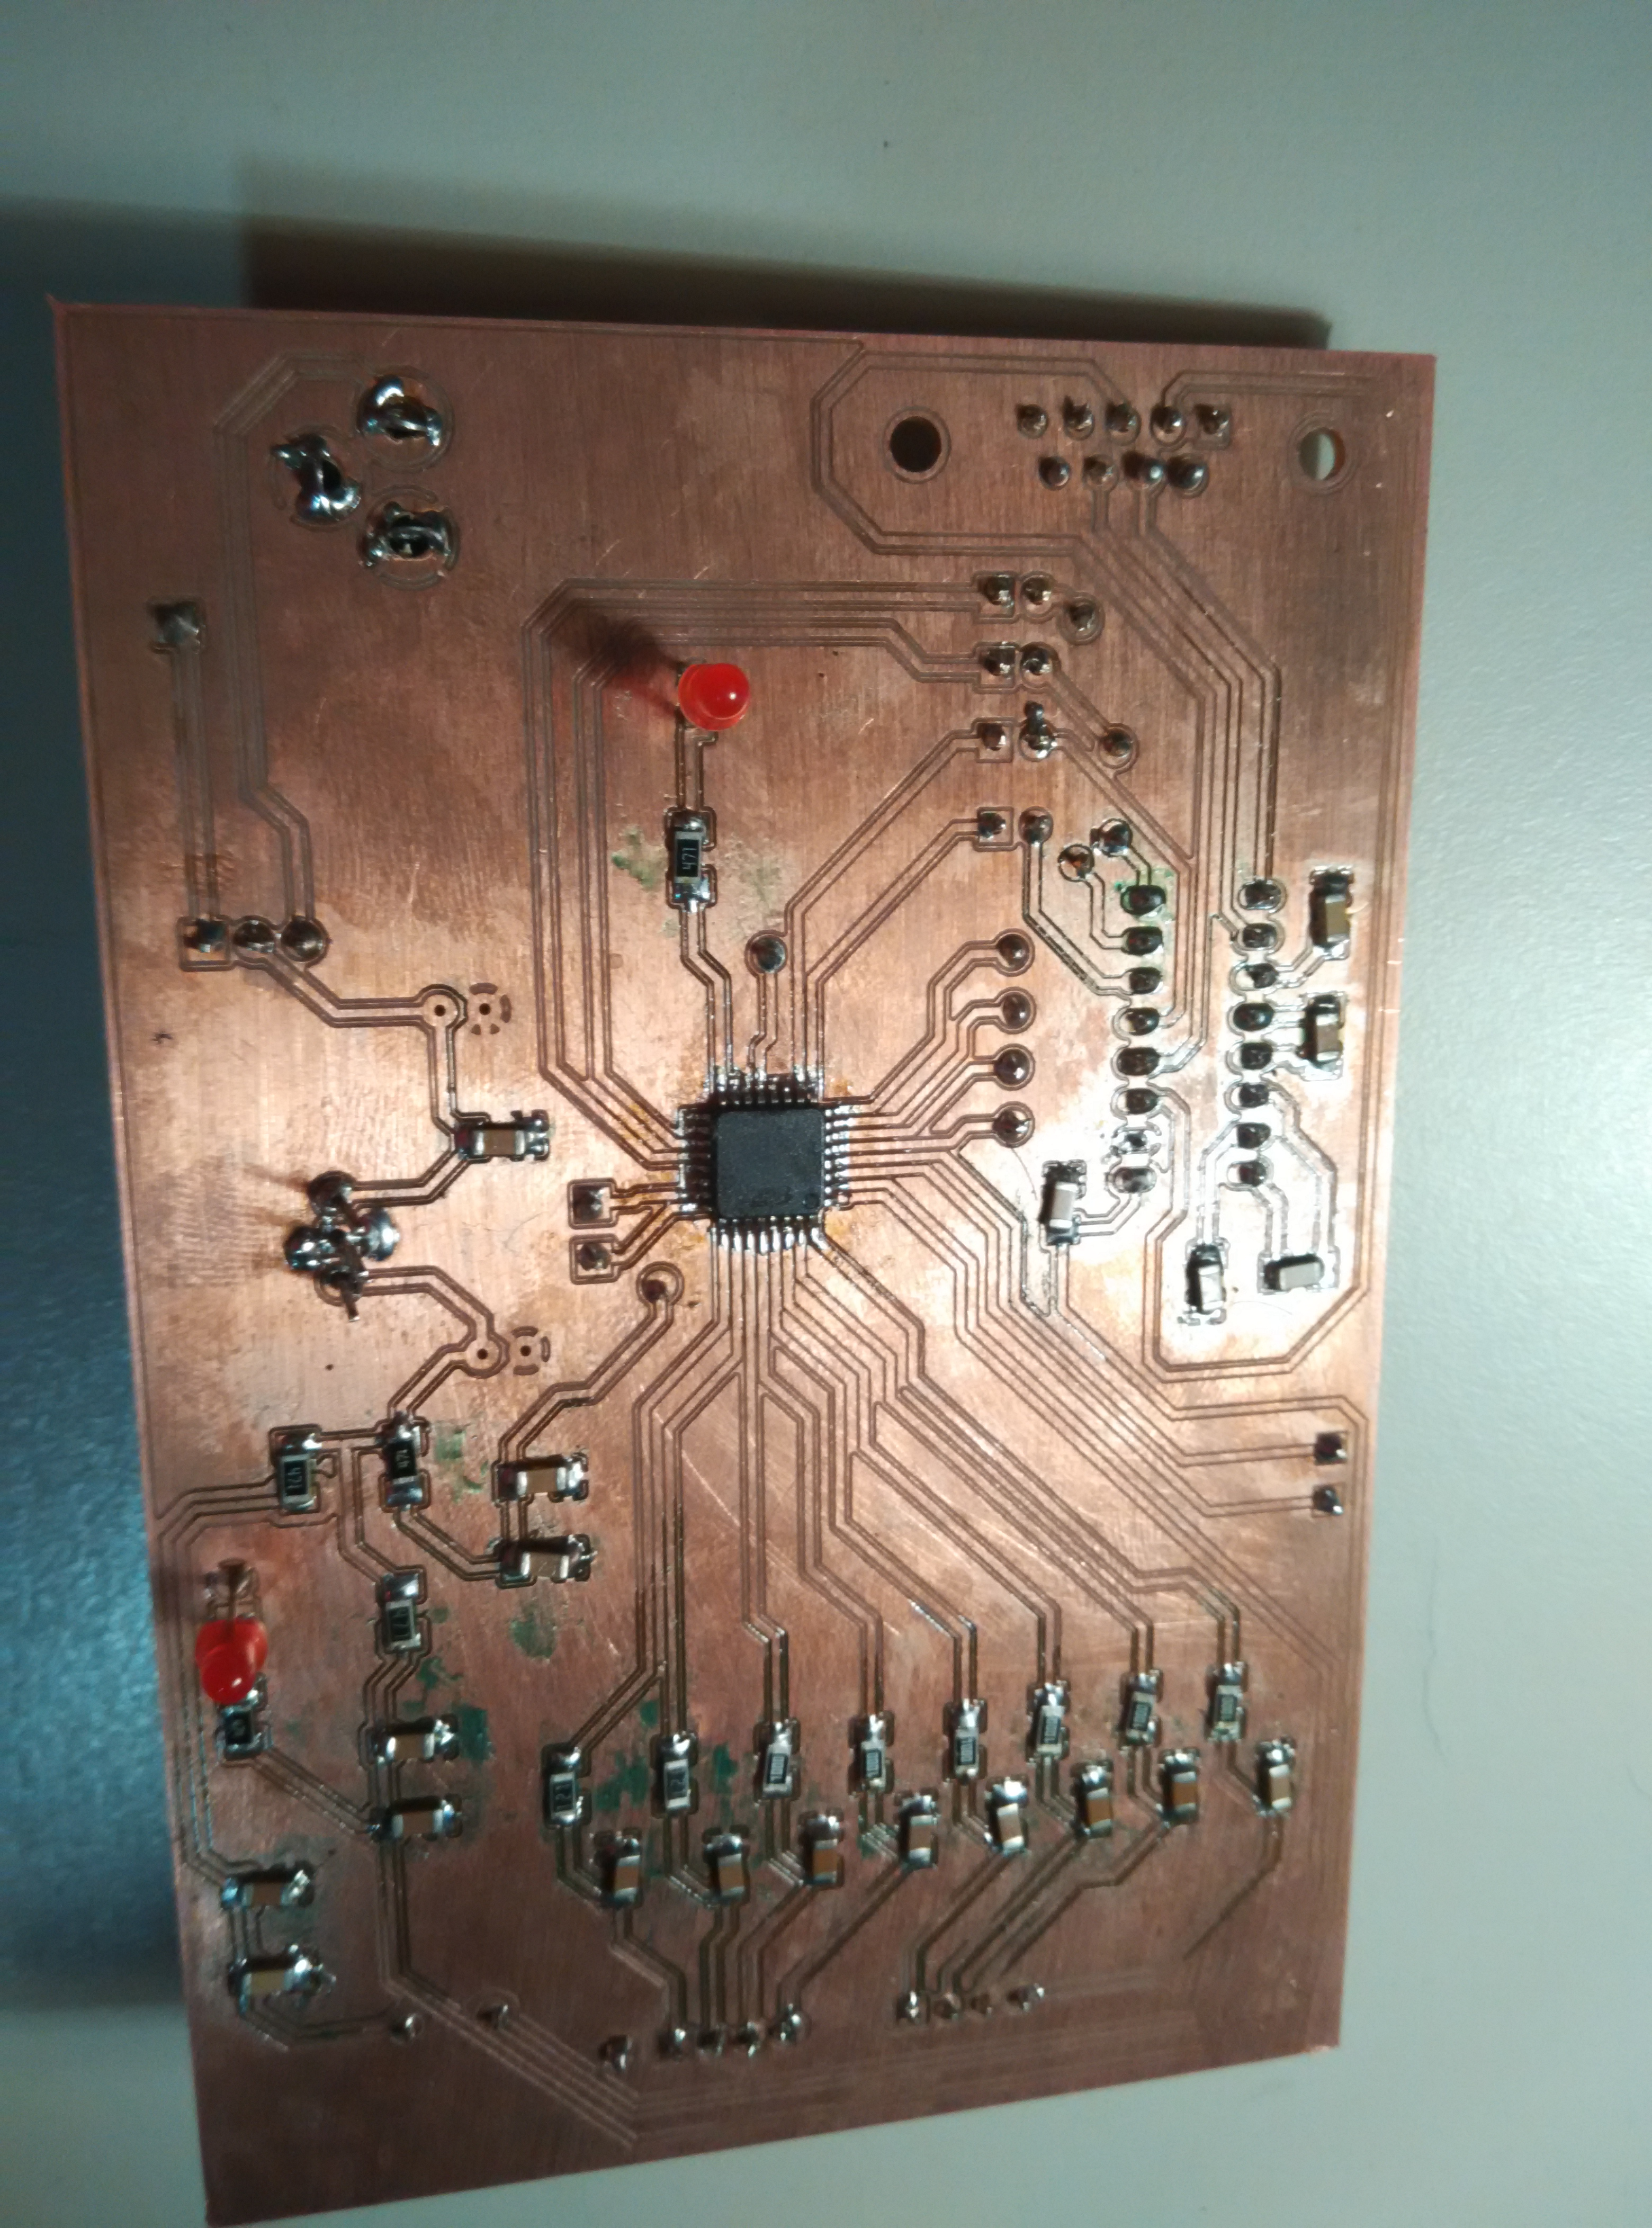
\includegraphics[width=0.80\textwidth, height = 10cm]{resultadohardware1}
  \caption{Placa completa con todo sus componentes soldados.}\label{fig:resultadohardware1}
\end{figure}

En esta iteración cumplimos con los siguientes requerimientos planteados:
\begin{itemize}
  \item Al circuito se le deben poder conectar 8 entradas analógicas.
  \item Al circuito se le deben poder conectar 4 entradas de eventos digitales externos.
  \item Las entradas analógicas deben tener filtros para mejorar la inmunidad al ruido.
  \item Se debe incluir en el diseño el circuito necesario para soportar comunicación vía RS232.
  \item La placa debería poder alimentarse a través de una fuente de tensión externa.
  \item Se debería poder conectar el debugger del microcontrolador a la placa para poder programarlo.
  \item El circuito de programación del microcontrolador debería estar separado la placa principal.
\end{itemize}

Viendo los resultados de las pruebas, puede verse que no fueron una sino varias las veces que fue necesario reimprimir la placa, hasta lograr que funcionara como era esperado. En cada nueva impresión, se mejoraban aspectos relacionados a su tamaño, la distribución de los componentes, y su robustez con respecto a los posibles cortocircuitos generados a partir de imperfecciones en el ruteo de pistas.

La Figura \ref{placaterminadait3} muestra el resultado de la placa al final de la iteración.

% section resultados (end)

% chapter iteracion_3 (end)

\chapter{Iteración 4: Diseño final del Software} % (fold)
\label{cha:iteracion_4}

\section{Introducción} % (fold)
\label{it5:sec:introduccion}

En esta iteración, se intentó dar un cierre a un primer prototipo de software que cumpla con todos los requerimientos, o la mayor cantidad posible, teniendo en cuenta el riesgo intrínseco de cada uno.

Al final de la iteración 2, en la sección \ref{it2:sec:conclusiones_de_la_iteracion_2}, se especifica una lista con requerimientos cumplidos. Nuestro punto de partida para continuar el desarrollo del programa es esta lista. 

El objetivo principal de esta iteración es conformar un programa que cumpla con todos los requerimientos funcionales, inherentes al software de la plataforma.

% section introduccion (end)

\section{Requerimientos de la iteración} % (fold)
\label{it5:sec:requerimientos_de_la_iteracion}

Los requerimientos de esta iteración están planteados en base a los requerimientos principales, y los resultados de las pruebas y el desarrollo de la iteración 2. Además, se incluyen requerimientos nuevos, que surgieron por propuesta nuestra o de nuestro director, con motivo de mejorar las prestaciones de la plataforma.

\begin{itemize}
\item Se deberían poder configurar tiempos de intervalo entre cada medición para cada canal por separado (deriva de 1.5)
\item Se deberían poder guardar las configuraciones actuales en la memoria flash del microcontrolador, para poder restablecerlas en caso que el sistema se apague y se vuelva a prender. [4.1]
\item Se debería generar una marca de tiempo relativa al inicio de conversiones en cada medición realizada. [4.2]
\item Los datos que se envían a la placa de gestión para cada medición debería incluir, además de la medición, el numero de pin o pines (si es modo diferencial) de donde se esta midiendo. [4.3]
\item Los datos que se envían a la placa de gestión para cada medición debería incluir, además de la medición, el modo de conversión del canal por donde se esta midiendo. [4.4]
\item Los datos que se envían a la placa de gestión para cada medición debería incluir, además de la medición, la marca de tiempo relativa correspondiente de la medición hecha. [4.5] 
\end{itemize}


% section requerimientos_de_la_iteracion (end)

\section{Desarrollo} % (fold)
\label{it5:sec:desarrollo}

Focalizamos el desarrollo del programa en obtener un prototipo final, preparado para que se ejecute de manera continua en la placa de instrumentación construida. En una primera instancia, terminamos aquellas funcionalidades ligadas a los requerimientos principales, y luego nos dedicamos a comprobar el funcionamiento del mismo, mediante unit-testing y tests de sistema.

La Figura \ref{it5:fig:bloquesquintaiteracion} muestra el diagrama de bloques del programa terminado, al final esta iteración. Si se compara con la Figura \ref{it2:fig:bloquesprimeraiteracionsoftware}, el cambio en la estructura no es significativo. El mayor cambio esta en las funciones dentro de los bloques. Hay funciones nuevas, funciones que sufrieron cambios y funciones que se eliminaron.

\begin{figure}[h]
  \centering
  \includegraphics[width=1\textwidth, height = 10cm]{bloquesquintaiteracion}
  \caption{}\label{it5:fig:bloquesquintaiteracion}
\end{figure}

\subsection{Conversor} % (fold)
\label{sub:conversor}

Las funciones del conversor se rediseñaron con el objetivo de lograr que el usuario pueda configurar tiempos de intervalos de mediciones en cada canal por separado.

En la sección \ref{it2:sub:el_modulo_conversor}, se explica el funcionamiento del buffer del conversor. Hasta el momento, el buffer poseía 8 posiciones, una por cada canal, con el objetivo de informar al programa el estado de ese canal. Estos estados son: inhabilitado, canal único, o canal diferencial.

\begin{figure}[h]
  \centering
  \includegraphics[width=0.80\textwidth, height = 7cm]{bufferdinamicovacio}
  \caption{Estado de los buffers en el momento en que se terminaron de configurar las distintas vías de conversión, pero aun no se activo el modo de conversión continua}\label{it5:fig:bufferdinamicovacio}
\end{figure}

En esta versión del programa, utilizamos dos buffers de 11 posiciones cada uno. A diferencia del buffer de conversión de la iteración 2, cada posición ya no representa un único canal sino que representa una "vía de conversión". Una vía de conversión es una fuente de telemetría que puede provenir de un canal único o diferencial.
De manera figurativa, podría decirse que un buffer es 'dinámico', y el otro es 'estático'. Similar al buffer de conversión de la iteración 2, el buffer estático determina si un canal esta habilitado o no. Además de esto, determina el valor del intervalo de mediciones de dicho canal. Si la posición que corresponde a ese canal contiene un 0, el canal esta inhabilitado; cualquier numero mayor a 0 indica que el canal esta habilitado. Si el canal esta habilitado, el numero puede estar en un rango de 1 a 65536, siendo este numero una medida del intervalo temporal que habrá entre cada medición cuando el sistema entre en modo de conversiones continuas. Mientras mayor es el numero, mayor es el intervalo entre cada medición para ese canal.
A diferencia del buffer original, el modo de conversión ya no se identifica con un numero, sino con la posición dentro del buffer, ya sea el estático o el dinámico. Las posiciones del 0 al 7 están reservadas para los 8 canales del conversor en modo canal único, y las posiciones del 8 al 11 son para los canales en modo diferencial. Las posiciones 8,9,10 y 11 representan a los pares de pines en modo diferencial (1,2); (3,4); (5,6) y (7,8) respectivamente. 


La secuencia para las conversiones funciona de la siguiente manera:

\begin{enumerate}
\item Cuando se configura el buffer, se establecen las vías de conversión con sus respectivos intervalos poniendo números de 1 a 65536 en los elementos del buffer estático.
\item Cuando se activa el modo de conversiones continuas, se realiza una copia del buffer estático para obtener el buffer dinámico, que es en realidad una instancia del buffer estático al comienzo de la conversiones continuas.
\item El programa itera sobre el buffer dinámico, decrementando los valores de cada elemento del buffer que no contenga un 0
\item Cuando se encuentra sobre un elemento que tiene valor igual a 1, es momento de obtener una medición de la vía de conversión ligada a esa posición.
\item Una vez habilitada la conversión para el canal, se copia el valor que se encuentra en el buffer estático para la misma posición en el buffer dinámico. Reiniciando la cuenta.
\end{enumerate}

La función que realiza la conversión, es ejecutada cada vez que se encuentra un 1 en una posición del buffer dinámico. Con el numero de posición del buffer, se sabe el numero de la vía de conversión por donde hay que convertir. Esta vía de conversión, como mencionamos anteriormente, puede ser de 0 a 11. En cada numero, se mide lo siguiente:

\begin{itemize}
\item 0 \textrightarrow  canal 0 modo único
\item 1 \textrightarrow  canal 1 modo único
\item 2 \textrightarrow  canal 2 modo único
\item 3 \textrightarrow  canal 3 modo único
\item 4 \textrightarrow  canal 4 modo único
\item 5 \textrightarrow  canal 5 modo único
\item 6 \textrightarrow  canal 6 modo único
\item 7 \textrightarrow  canal 7 modo único
\item 8 \textrightarrow  canal 0,1 modo diferencial
\item 9 \textrightarrow  canal 1,2 modo diferencial
\item 10 \textrightarrow  canal 2,3 modo diferencial
\item 11 \textrightarrow  canal 3,4 modo diferencial
\end{itemize}

Se tomaron las medidas suficientes, dentro del programa, para no permitir al usuario que establezca una configuración donde provoque que se solapen las vías de conversión con respecto a los canales. 

\begin{figure}[h]
  \centering
  \includegraphics[width=0.80\textwidth, height = 7cm]{bufferdinamicolleno}
  \caption{Estado de los buffers en el momento que se activa la conversión continua. Cada vez que un valor del buffer dinámico llega a 1, se restablece usando el buffer estático como referencia.}\label{it5:fig:bufferdinamicolleno}
\end{figure}

El numero dentro de cada posición representa el tiempo del intervalo. El intervalo mas corto es 1, y el mas largo es 65536. Los tiempos en segundos con respecto a los intervalos siguen una escala lineal, pero necesaria de calibrar en caso de ser necesaria una mayor precisión. Para mejorar la practicidad a la hora de establecer intervalos, conformamos una tabla con valores de intervalos nominales. A partir de dicha tabla, elaboramos un gráfico que se muestra en la Figura \ref{it5:fig:relacionintervalotiempo}.

\begin{table}[h]
\centering
\caption{Tabla con mediciones de tiempo para distintos valores de intervalos.}
\label{it5:tab:tablamediciones}
\begin{tabular}{|l|l|}
\hline
\rowcolor[HTML]{34CDF9} 
Intervalo & Tiempo (s) \\ \hline
\rowcolor[HTML]{CBF3FF} 
9         & 1          \\ \hline
\rowcolor[HTML]{CBF3FF} 
28        & 3          \\ \hline
\rowcolor[HTML]{CBF3FF} 
55        & 6          \\ \hline
\rowcolor[HTML]{CBF3FF} 
92        & 10         \\ \hline
\rowcolor[HTML]{CBF3FF} 
138       & 15         \\ \hline
\end{tabular}
\end{table}

\begin{figure}[h]
  \centering
  \includegraphics[width=0.80\textwidth, height = 7cm]{relacionintervalotiempo.JPG}
  \caption{Gráfico elaborado a partir de la tabla \ref{it5:tab:tablamediciones}, obtenido midiendo el tiempo entre cada medición para los intervalos en el eje de las abscisas. Observando la curva, llegamos a la conclusión que los distintos valores de tiempo correspondientes a los intervalos se comportan de manera lineal. Haciendo una extrapolación básica, podemos decir que el intervalo mas largo, con un valor de 65536, corresponde a un tiempo de aproximadamente 2 horas entre cada medición.}\label{it5:fig:relacionintervalotiempo}
\end{figure}

Las funciones "cambiar\_pin" y "analizar\_buffer" dentro del modulo de conversor, manejan los buffers y realizan las conversiones según las configuraciones. Ambas son ejecutadas cíclicamente en el modo de conversiones continuas. "cambiar\_pin" prepara el hardware del conversor según cual es el canal próximo a medir, y "analizar\_buffer" recorre el buffer, habilitando o no la conversión, y actualizándolo en cada corrida. Las figuras \ref{it5:fig:actividadanalizarbuffer} y \ref{it5:fig:actividadcambiarpin} describen las funciones con diagramas de actividad.
 
\begin{figure}[h]
  \centering
  \includegraphics[width=1\textwidth, height = 12cm]{actividadanalizarbuffer}
  \caption[Diagrama de actividad de la función analizar buffer]{Diagrama de actividad que muestra el funcionamiento de la función analizar buffer. Esta función esta pensada para trabajar junto con "cambiar\_pin". En cada cambio de pin, se analiza el buffer para saber si hay que convertir o no, y actualizar el estado de los elementos del buffer, que corresponden en uno a uno con todas las vías de conversión posibles.}\label{it5:fig:actividadanalizarbuffer}
\end{figure}



\begin{figure}[h]
  \centering
  \includegraphics[width=1\textwidth, height = 12cm]{actividadcambiarpin}
  \caption[Diagrama de actividad de la función cambiar pin]{Diagrama de actividad que ilustra la lógica dentro de la función cambiar\_pin, dentro del modulo del conversor. Esta función es llamada luego de cada conversión. En cada llamado, se selecciona un nuevo canal a medir. No discrimina si el canal esta o no habilitado para medir, en caso en que no lo este, se llamara inmediatamente para cambiar el pin nuevamente sin realizar medición alguna.}\label{it5:fig:actividadcambiarpin}
\end{figure}

\subsubsection{Marca de tiempo} % (fold)
\label{ssub:marca_de_tiempo}

En algunos casos, puede ser necesario saber la hora, minuto y segundo en el que se midió. Para esto, sugerimos la idea de que se incluya una marca de tiempo dentro de los meta-datos enviados a la placa de gestión. Fue un requerimiento propuesto por nosotros en una etapa ya avanzada del proyecto. Esta marca de tiempo es necesariamente relativa al momento de inicio de conversiones continuas. Esto se debe a que la placa de instrumentación no tiene manera directa de calcular la fecha y hora exacta del día, por lo que obtener una marca de tiempo absoluta de manera directa en esta placa no es practico. 
La solución planteada para obtener una marca de tiempo absoluta fue calculándola en la placa de gestión. Al estar esta placa conectada a internet, puede obtener fácilmente la fecha y hora de inicio de conversiones. Con esto, a la fecha y hora se le suma la marca relativa de cada medición, y se obtiene así la marca de tiempo absoluta. Sabiendo esto, en esta sección explicamos la obtención de la marca de tiempo relativa. La marca de tiempo absoluta se obtiene usando la marca relativa junto con la fecha y hora actuales. Implica que deberá calcularse en un sistema con posibilidad de obtener esta información \\

El proceso para obtener la marca de tiempo esta descripto en la imagen \ref{it5:fig:secuenciaobtenermarca} mediante un diagrama de secuencia. La marca de tiempo relativa se obtiene con el uso del timer2. Esto significa reducir la cantidad de contadores de eventos disponibles de 2 a 1, lo cual afecta de manera directa a un requerimiento principal. La solución planteada fue dejar como opcional el calculo de la marca de tiempo, pudiendo así elegir el uso del timer2 entre contador de eventos o contador interno para la marca de tiempo. Esto es posible porque hay casos donde no es necesario ser preciso a la hora de tener el tiempo de las mediciones, y se pueden calcular las marcas directamente desde el sistema de gestión, y así dejar libre al Timer2 para el conteo de eventos. Esto fue un compromiso dado el estado avanzado del proyecto.


\begin{figure}[h]
  \centering
  \includegraphics[width=1\textwidth, height = 9cm]{secuenciaobtenermarca}
  \caption[Diagrama de secuencia para la obtención de una marca de tiempo]{Diagrama de secuencia que muestra la interacción entre el conversor y Timer 2 para obtener la marca de tiempo. En el diagrama, la marca de tiempo esta representada mediante un objeto que alberga un único campo, que es la marca de tiempo. En cada interrupción de Timer 2 este valor se actualiza, y en cada conversión se obtiene el valor actual para enviarlo junto con la medición obtenida en la conversión.}\label{it5:fig:secuenciaobtenermarca}
\end{figure}

% subsubsection marca_de_tiempo (end)

% subsection conversor (end)

\subsection{Interfaz de usuario} % (fold)
\label{it5:sub:interfaz_de_usuario}

La interfaz de usuario siguió un diseño parecido al descrito en la sección \ref{it2:sub:logica_de_las_funciones_de_la_interfaz}. Gracias al diseño de la interfaz, agregar nuevos comandos con nuevos argumentos fue sencillo, siempre y cuando se respete la expresión regular.

Los comandos disponibles al final de esta iteración fueron:

\begin{itemize}
  \item SSE: - \textit{set single ended}: Establece un canal en modo único.
  \item SDI: - \textit{set differential}: Establece un par de canales en modo diferencial.
  \item GSE: - \textit{get single ended}: Obtiene una conversión instantánea en modo canal unico sobre un canal.
  \item GDI: - \textit{get differential}: Obtiene una conversión instantánea en modo diferencial sobre un par de canales.
  \item GDI: - \textit{get differential}: Obtiene una conversión instantánea en modo diferencial sobre un par de canales.
  \item SGA: - \textit{set gain}: Establece el nivel de ganancia del conversor.
  \item GT0: - \textit{get timer 0}: Obtiene el valor actual de la cuenta de timer 0, configurado como contador de eventos.
  \item GT2: - \textit{get timer 2}: Obtiene el valor actual de la cuenta de timer 2, configurado como contador de eventos.
  \item SHA: - \textit{show configuration}: Muestra la configuración actual de todos los canales y la ganancia del conversor.
  \item ST: - \textit{start}: Inicia el modo de conversiones continuas.
\end{itemize}

El conjunto entero de comandos esta documentado con mayor detalle en el apéndice \ref{ap:instrucciones}.
% subsection interfaz_de_usuario (end)

\subsection{Memoria flash} % (fold)
\label{it5:sub:memoria_flash}

La memoria flash del microcontrolador puede ser utilizada para guardar las configuraciones actuales, de forma que si el sistema se apaga, se pueda volver a iniciar con las configuraciones ya cargadas, sin necesidad de volver a establecer todo cada vez que se inicie nuevamente. Esto fue planteado como requerimiento para esta iteración, pero no pudo ser posible. Las operaciones necesarias para leer y escribir la memoria y el tamaño de la misma hicieron que sea difícil realizar la escritura y la lectura de la misma.

Tanto el programa que corre en el microprocesador como los datos de configuración debe guardarse en la misma memoria flash de 8Kb, siendo que el programa ocupa alrededor de 7Kb. En el Kb que resta, es posible guardar las configuraciones, pero el método de escritura de la flash pone en riesgo la integridad del programa. La única manera de escribir en memoria es haciéndolo sobre una pagina de 512 bytes. Dado el reducido espacio disponible, era probable que en una escritura se sobre escribiera parte del programa, haciendo que el sistema falle.
Teniendo en cuenta esto, se decidió no utilizar la flash para guardar las configuraciones. Por lo tanto, cada vez que el sistema se apague, se pierden las configuraciones, sin posibilidad de guardarlas.

% subsection memoria_flash (end)

% section desarrollo (end)

\section{Pruebas} % (fold)
\label{it5:sec:pruebas}

\begin{table}[h]
\centering
\caption{Test de sistema 1: Comportamiento esperado del conversor}
\label{it5:tab:testsistema1}
\begin{tabular}{p{2cm} p{9cm}}
\multicolumn{2}{c}{\cellcolor[HTML]{68CBD0}{\color[HTML]{000000} Prueba de sistema}} \\
Prueba \#        & 3 \\
\hline
Nombre           & Comportamiento esperado del conversor \\
\hline
Requerimiento & 1.5 \\
\hline
Descripción      & Con esta prueba, se comprueba que el sistema permite establecer intervalos de medición individuales para cada canal, y que se comporta de manera consistente con el el paso del tiempo. \\
\hline
Pre-condiciones  & \tabitem Sistema configurado con dos pines en modo canal único \\
                 & \tabitem Un canal esta configurado con un tiempo de 1 y otro con 50 \\
                 & \tabitem Generadores de tensión conectados a los pines configurados  \\
                 & \tabitem Computadora conectada al sistema mediante cable serial RS-232 \\
                 & \tabitem Lector de canal serial abierto en la computadora  \\
                 & \tabitem Sistema midiendo en modo de conversiones continuas\\
\hline

Post-condiciones & La frecuencia de medición para el canal en 1 debería ser mayor a la frecuencia del canal en 50.                     
\\
\hline
Secuencia  & \tabitem Establecimos una tensión de 1,5 voltios en el primer generador, conectado al canal con intervalo 1 y una de 2 voltios en el segundo, con intervalo 50 \\
\hline
Resultados       & El canal con intervalo 1 tenia una frecuencia mucho mayor al canal con intervalo 50, que era lo esperado. La relación entre las frecuencias parecía ser lineal (50 veces mas frecuente el primero que el segundo), aunque no teníamos una manera precisa de medirlo, mas que contar la cantidad de mediciones en un intervalo grande de tiempo.
\end{tabular}
\end{table}

\begin{table}[h]
\centering
\caption{Test de sistema 2: Generación de la marca de tiempo}
\label{it5:tab:testsistema2}
\begin{tabular}{p{2cm} p{9cm}}
\multicolumn{2}{c}{\cellcolor[HTML]{68CBD0}{\color[HTML]{000000} Prueba de sistema}} \\
Prueba \#        & 3 \\
\hline
Nombre           & Generación de la marca de tiempo \\                 
\hline
Requerimiento & 4.2 \\
\hline
Descripción      & En cada conversión, se debería registrar una marca de tiempo con un numero que hace referencia al tiempo que transcurrió desde el momento que se iniciaron las conversiones al momento donde se toma la medición. \\
\hline
Pre-condiciones  & \tabitem Sistema configurado con un pin en modo canal único, con un intervalo de 9, que corresponde a 1 segundo según la tabla \ref{it5:tab:tablamediciones} \\
                 & \tabitem Generador de tensión conectado al pin configurado  \\
                 & \tabitem Computadora conectada al sistema mediante cable serial RS-232 \\
                 & \tabitem Lector de canal serial abierto en la computadora  \\
                 & \tabitem Cronometro en 00:00\\
                 & \tabitem Reloj en hora\\
\hline

Post-condiciones & La diferencia entre cada marca de tiempo y la siguiente debería ser constante, y debería ser aproximada al valor en segundos dado por el intervalo. El calculo en fecha y hora de la ultima marca de tiempo y el valor del cronometro (hecho con ayuda del reloj) debería dar aproximadamente igual. \\
\hline
Secuencia  & \tabitem Establecimos una tensión en el generador. \\
           & \tabitem Iniciamos las conversiones continuas. \\
           & \tabitem Dimos arranque al cronometro. \\
           & \tabitem Medimos el tiempo entre cada medición con ayuda del cronometro en 30 mediciones sucesivas. \\

Resultados       & Los resultados fueron los esperados. El intervalo de tiempo entre cada medición era aproximadamente 1 segundo en todos los casos. Lo que significa que el tiempo entre cada medición no varia con el paso del tiempo para un intervalo constante. 
\end{tabular}
\end{table}

\begin{table}[h]
\centering
\caption{Test de sistema 3: Formato esperado del mensaje}
\label{it5:tab:testsistema3}
\begin{tabular}{p{2cm} p{9cm}}
\multicolumn{2}{c}{\cellcolor[HTML]{68CBD0}{\color[HTML]{000000} Prueba de sistema}} \\
Prueba \#        & 3 \\
\hline
Nombre           & Formato esperado del mensaje \\                     
\hline
Requerimiento    & 4.3, 4.4, 4.5 \\
\hline
Descripción      & Cada dato que se envía a la placa de gestión incluye la siguiente información: Medición, pin, modo, marca de tiempo. Estos datos están enviados con un formato especial, y se envían en simultaneo. Esta prueba verifica que cada mensaje contenga el formato correcto y que los datos sean coherentes a las configuraciones. \\
\hline
Pre-condiciones  & \tabitem Sistema configurado con el pin 3 en modo canal único, con un intervalo de 10 \\
                 & \tabitem Generador de tensión conectado al pin configurado con un valor de 1,5 volts  \\
                 & \tabitem Computadora conectada al sistema mediante cable serial RS-232 \\
                 & \tabitem Lector de canal serial abierto en la computadora  \\
                 & \tabitem Sistema midiendo en modo de conversiones continuas\\
\hline

Post-condiciones & El mensaje recibido en el lector serial debería ser "1500,3,SE,[marca de tiempo]".                     
\\
\hline
Resultados       & El formato era correcto
\end{tabular}
\end{table}

% section pruebas (end)

\section{Conclusiones} % (fold)
\label{sec:conclusiones}

Algunos de los requerimientos principales y secundarios no se llegaron a cumplir por inconvenientes en el desarrollo, pero se tomaron ciertas medidas para compensar los problemas, sobretodo en aquellos que involucraban a los requerimientos principales y de mayor riesgo.

\begin{itemize}
\item Guardar las configuraciones y parámetros del programa en la memoria flash no fue posible debido al poco espacio dentro de la memoria, y la impracticidad del método de escritura y lectura. Este no era un requerimiento principal, por lo que simplemente lo descartamos.
\item La cantidad de contadores posibles paso de cuatro a dos, o solo uno si se utiliza la funcionalidad de la marca de tiempo. Los 4 contadores eran un requerimiento principal. En la iteración 4, diseñamos y construimos un PCB en doble faz, que contiene los dos circuitos de la plataforma idénticos en cada lado, obteniendo dos plataformas y duplicando la cantidad de recursos. Esto da un total de 4 contadores utilizables, con la marca de tiempo inhabilitada en ambas plataformas. 
\end{itemize}

A pesar de esto, el software de la plataforma es estable, robusto y funcional. Los tests unitarios aseguran la respuesta necesaria ante cualquier error por parte del usuario. Además, el hecho que no sea un software de gran tamaño permite que no se cuelgue en medio de una ejecución, interrumpiendo una sesión de adquisición de datos. A continuación listamos las funcionalidades principales desarrolladas, en esta iteración, según los requerimientos principales.

\begin{itemize}
\item Es posible configurar tiempos de intervalo entre cada medición para cada canal por separado (cumple con 1.5)
\item Los datos que se envían a la placa de gestión para cada medición incluyen, además de la medición, el numero de pin o pines (si es modo diferencial) de donde se esta midiendo. (cumple con 4.3)  
\item Los datos que se envían a la placa de gestión para cada medición incluyen, además de la medición, el modo de conversión del canal por donde se esta midiendo. (cumple con 4.4)
\item Los datos que se envían a la placa de gestión para cada medición incluyen, además de la medición, la marca de tiempo relativa correspondiente de la medición hecha. (cumple con 4.5)
\end{itemize}

El requerimiento 4.1 no pudo ser cumplido debido a complicaciones con el modulo flash del microcontrolador, y se probara el cumplimiento del requerimiento 4.2 cuando se cuente con un sistema embebido que pueda generar marcas de tiempo absolutas.

% section conclusiones (end)

% chapter iteracion_4 (end)

\chapter{Iteracion 5: Diseño final del Software} % (fold)
\label{cha:iteracion_5}

\section{Introduccion} % (fold)
\label{it5:sec:introduccion}

En este capitulo, se describe el desarrollo de la segunda itearacion de software. Hasta el momento, tenemos un programa embebido en el microcontrolador que cumple con los requerimientos especificados en la seccion \ref{it2:sub:estado_de_los_requerimientos}. En esta iteracion, los objetivos fueron principalmente orientados a profundizar las funciones del conversor para que se puedan establecer intervalos individuales entre cada medicion para cada canal. Ademas, se intento incluir a SMBus como alternativa de interfaz serial, que hasta el momento era unicamente UART. Se propuso tambien utilizar el modulo flash del microcontrolador con el objetivo de guardar las configuraciones una vez establecidas, de manera que no sea necesario volver a configurar el sistema en cada encendido.

% section introduccion (end)

\section{Requerimientos de la iteracion} % (fold)
\label{it5:sec:requerimientos_de_la_iteracion}

De los requerimientos principales y el estado del programa al final de la iteracion 2 (cpitulo \ref{cha:iteracion_2}), se proponen los siguientes requerimientos para el programa:

\begin{itemize}
\item Se deberian poder configurar tiempos de intervalo entre cada medicion para cada canal por separado
\item Se deberian poder guardar las configuraciones actuales en la memoria flash del microcontrolador, para poder reestablecerlas en caso que el sistema se apague y se vuelva a prender.
\item Se deberia utilizar SMBus ademas de UART para transmitir los datos de la placa de instrumentacion a la placa de gestion.
\item Todas las funcionalidades del sistema deberian estar testeadas utilizando unit-testing y realizando pruebas de sistema.
\end{itemize}


% section requerimientos_de_la_iteracion (end)

\section{Desarrollo} % (fold)
\label{it5:sec:desarrollo}

Ademas de explicar las modificaciones hechas a los modulos del programa para que cumplan con los requerimientos de la iteracion, mencionaremos todos los modulos que han tenido cambios, influyan o no en los requerimientos. El objetivo es dar una idea de la actualizacion del programa embebido. 

\subsection{Logica para permitir intervalos individuales de medicion: Buffer de conversion estatico y dinamico} % (fold)
\label{it5:sub:logica_para_permitir_intervalos_individuales_de_medicion_buffer_de_conversion_estatico_y_dinamico}

En esta seccion, ocupamos el rediseño de las funciones del conversor con el objetivo de lograr que el usuario pueda configurar tiempos de intervalos de mediciones en cada canal por separado. El tiempo entre cada medicion no es menor, dado que dependiendo el tipo de sensor, puede necesitarse que las mediciones sean de frecuencia alta o baja.

En la seccion \ref{sub:logica_de_las_funciones_del_conversor}, se explica el funcionamiento del buffer del conversor. Este buffer posee 8 posiciones, una por cada canal, con el objetivo de informar al programa el estado de ese canal. Estos estados son: inhabilitado, canal unico, diferencial.

En esta version, se utilizan dos buffers de 11 posiciones cada uno. Cada posicion ya no representa un unico canal sino que representa una via de conversion. Elaboraremos esto mas adelante. Estos buffers pueden diferenciarse uno del otro en que uno puede decirse que es "estatico", y el otro "dinamico". De la misma manera que el buffer original, el buffer estatico determina si un canal esta habilitado o no: Si la posicion que corresponde a ese canal contiene un 0, entonces ese canal esta habilitado. Cualquier numero distinto de 0 indica que el canal esta habilitado. A diferencia del buffer original, el modo de conversion ya no se identifica con un numero, sino con la posicion dentro del buffer, ya sea estatico o dinamico. Las posiciones del 0 al 7 estan reservadas para los 8 canales del conversor en modo canal unico, y las posiciones del 8 al 11 son para el modo diferencial. 
El contenido de cada elemento en el buffer es un numero que va de 1 a 255, en el caso en que este habilitado. Ese numero representa el tiempo que existe entre cada medicion. Mientras mayor es el numero, mayor es el intervalo entre mediciones. Esto funciona de la siguiente manera:

\begin{enumerate}
\item Cuando se configura el buffer, se establecen las vias de conversion con sus respectivos intervalos poniendo numeros de 1 a 255 en elementos del buffer estatico.
\item Cuando se activa el modo de conversiones continuas, se realiza una copia del buffer estatico para obtener el buffer dinamico, que es en realidad una instancia del buffer estatico al comienzo de la conversion continua.
\item El programa itera sobre el buffer dinamico, decrementando los valores de cada elemento del buffer que no contenga un 0
\item Cuando se encuentra sobre un elemento que tiene valor igual a 1, le avisa al programa que el proximo canal a medir es el actual.
\item Luego de esto, copia el valor que se encuentra en el buffer estatico para la misma posicion en la que se encuentra, para seguir con el proximo elemento.
\end{enumerate}


\begin{figure}[h]
  \centering
  \includegraphics[width=0.80\textwidth, height = 7cm]{bufferdinamicovacio}
  \caption{Estado de los buffers en el momento en que se terminaron de configurar las distintas vias de conversion, pero aun no se activo el modo de conversion continua}\label{fig:bufferdinamicovacio}
\end{figure}


\begin{figure}[h]
  \centering
  \includegraphics[width=0.80\textwidth, height = 7cm]{bufferdinamicolleno}
  \caption{Estado de los buffers en el momento que se activa la conversion continua. Cada vez que un valor del buffer dinamico llega a 1, se reestablece usando el buffer estatico como referencia.}\label{fig:bufferdinamicolleno}
\end{figure}

La funcion que se encarga de realizar las conversion, es disparada cada vez que se encuentra un 1 en una posicion del buffer dinamico. Con el numero de posicion del buffer, sabe el numero de la via de conversion por donde hay que convertir. Esta via de conversion, como mencionamos anteriormente, puede ser de 0 a 11. En cada numero, se mide lo siguiente:

\begin{itemize}
\item 0 \textrightarrow  canal 0 modo unico
\item 1 \textrightarrow  canal 1 modo unico
\item 2 \textrightarrow  canal 2 modo unico
\item 3 \textrightarrow  canal 3 modo unico
\item 4 \textrightarrow  canal 4 modo unico
\item 5 \textrightarrow  canal 5 modo unico
\item 6 \textrightarrow  canal 6 modo unico
\item 7 \textrightarrow  canal 7 modo unico
\item 8 \textrightarrow  canal 0,1 modo diferencial
\item 9 \textrightarrow  canal 1,2 modo diferencial
\item 10 \textrightarrow  canal 2,3 modo diferencial
\item 11 \textrightarrow  canal 3,4 modo diferencial
\end{itemize}


Se tomaron las medidas suficientes, dentro del programa, para no permitir al usuario que establezca una configuracion donde provoque que se solapen las vias de conversion con respecto a los canales. 

Las funciones "cambiar\_pin" y "analizar\_buffer" dentro del modulo de conversor, manejan los buffers y realizan las conversiones segun las configuraciones. Ambas son ejecutadas ciclicamente en el modo de conversiones continuas. "cambiar\_pin" prepara el hardware del conversor segun cual es el canal proximo a medir, y "analizar\_buffer" recorre el buffer, habilitando o no la conversion, y actualizandolo en cada corrida. Las figuras \ref{fig:actividadanalizarbuffer} y \ref{fig:actividadcambiarpin} describen las funciones con diagramas de actividad.
 
\begin{figure}[h]
  \centering
  \includegraphics[width=0.80\textwidth, height = 7cm]{actividadanalizarbuffer}
  \caption[Diagrama de actividad de la funcion analizar buffer]{Diagrama de actividad que muestra el funcionamiento de la funcion analizar buffer. Esta funcion esta pensada para trabajar junto con "cambiar\_pin". En cada cambio de pin, se analiza el buffer para saber si hay que convertir o no, y actualizar el estado de los elementos del buffer, que corresponden en uno a uno con todas las vias de conversion posibles.}\label{fig:actividadanalizarbuffer}
\end{figure}



\begin{figure}[h]
  \centering
  \includegraphics[width=0.80\textwidth, height = 7cm]{actividadcambiarpin}
  \caption[Diagrama de actividad de la funcion cambiar pin]{Diagrama de actividad que ilustra la logica dentro de la funcion cambiar\_pin, dentro del modulo del conversor. Esta funcion es llamada luego de cada conversion. En cada llamado, se selecciona un nuevo canal a medir. No discrimina si el canal esta o no habilitado para medir, en caso en que no lo este, se llamara inmediatamente para cambiar el pin nuevamente sin realizar medicion alguna.}\label{fig:actividadcambiarpin}
\end{figure}

% subsection logica_para_permitir_intervalos_individuales_de_medicion_buffer_de_conversion_estatico_y_dinamico (end)

\subsection{Interfaz de usuario} % (fold)
\label{it5:sub:interfaz_de_usuario}

La interfaz de usuario siguio un diseño parecido al terminado en la iteteracion \ref{iteracion_2}. Agregarle funcionailidades es simple gracias al diseño de la interfaz. Cada vez que exista una funcionalidad nueva, hay que conformar un nuevo comando e incluirlo en el espacio de nombres.

Los comandos disponibles al final de esta iteracion son:

\begin{itemize}
  \item SSE: - \textit{set single ended}: Establece un canal en modo unico.
  \item SDI: - \textit{set differential}: Establece un par de canales en modo diferencial.
  \item GSE: - \textit{get single ended}: Obtiene una conversion instantanea en modo canal unico sobre un canal.
  \item GDI: - \textit{get differential}: Obtiene una conversion instantanea en modo diferencial sobre un par de canales.
  \item GDI: - \textit{get differential}: Obtiene una conversion instantanea en modo diferencial sobre un par de canales.
  \item SGA: - \textit{set gain}: Establece el nivel de ganancia del conversor.
  \item GT0: - \textit{get timer 0}: Obtiene el valor actual de la cuenta de timer 0, configurado como contador de eventos.
  \item GT2: - \textit{get timer 2}: Obtiene el valor actual de la cuenta de timer 2, configurado como contador de eventos.
  \item SHA: - \textit{show configuration}: Muestra la configuracion actual de todos los canales y la ganancia del conversor.
  \item ST: - \textit{start}: Inicia el modo de conversiones continuas.
\end{itemize}

Estas funciones estan descriptas con detalle en el apendice \ref{ap:instrucciones}.
s
% subsection interfaz_de_usuario (end)

\subsection{Memoria flash} % (fold)
\label{it5:sub:memoria_flash}

En esta iteracion, surgio la idea de utilizar la memoria flash del microcontrolador para guardar las configuraciones actuales, de forma que si el sistema se apaga, se pueda volver a iniciar con las configuraciones ya cargadas, sin necesidad de volver a establecer todo cada vez que se inicie nuevamente. Pero esto no pudo ser posible, las operaciones necesarias para leer y escribir la memoria y el tamaño de la misma hicieron que sea difícil realizar la escritura y la lectura de la misma. Para escribir una palabra en memoria, es necesario borrar toda la pagina en donde se encuentra la palabra para luego reescribirla. Cada pagina de la memoria flash ocupa 512 Bytes.

Tanto el programa que corre en el microprocesador como los datos de configuración debe guardarse en la misma memoria flash de 8Kb. El programa ocupa alrededor de 7Kb. En el Kb que sobra, es posible guardar las configuraciones, pero lo que lo dificulta es que el método de escritura de la flash pone en riesgo la integridad del programa. Teniendo en cuenta esto, se decidió no utilizar la flash para guardar las configuraciones. Por lo tanto, cada vez que el sistema se apague, se pierden las configuraciones, sin posibilidad de guardarlas.

% subsection memoria_flash (end)

% section desarrollo (end)

\section{Pruebas} % (fold)
\label{it5:sec:pruebas}

% section pruebas (end)

\section{Resultados} % (fold)
\label{it5:sec:resultados}

% section resultados (end)

% chapter iteracion_5 (end)

\chapter{Iteracion 6: Caso de prueba con un sensor de campo electrostatico} % (fold)
\label{cha:iteracion_6}

\section{Introduccion} % (fold)
\label{it6:sec:introduccion}

Parte de este proyecto fue poner a prueba nuestro sistema utilizando un sensor detector de campo electrostatico. Ademas de obtener las mediciones, fue necesario realizar un sistema de control para el motor del sensor. En esta iteracion realizamos la adaptacion necesaria de los requisitos de funcionamiento del sensor a nuestro sistema de instrumentacion, probando asi el funcionamiento del mismo, asi como tambien el funcionamiento del sistema gestionador desarrollado en la iteracion \ref{cha:iteracion_6} 

\subsection{Marco teorico} % (fold)
\label{it6:sub:marco_teorico}

La intensidad de un campo electrico se puede medir, en principio, colcando un medidor de voltaje entre dos placas metalicas paralelas separadas por una distancia. El problema de esto es que, como el medidor de voltaje suele tener una impedancia alta en la entrada, cualquier voltaje inducido en las placas se pierde rapidamente, y no podria usarse para medir el capo electrico. Para arreglar esto, se utiliza la tecnica de las aspas. Se coloca una placa conductora, y sobre la misma se posiciona un sistema con aspas de forma que cuando estas roten, se cubra y se exponga periodicamente la placa conductora al campo electrico ambiental. Para lograr esto apropiadamente, el rotor que hace girar las aspas debe estar conectado a tierra. La placa conductora esta conectada a tierra a traves de un amplificador de transconductancia, que convierte la corriente que va desde la placa a tierra en una tension. \\

A medida que la placa conductora este expuesta al campo electrico, el campo induce una corriente a tierra mientras que atrae o repele la carga de la placa conductora. A medida que la placa esta cubierta del campo electrico, la carga inducida se drena. Entonces las placas inducen una corriente alterna a masa que es proporcional a la intensidad del campo electrico estatico. Esta corriente alterna luego puede ser rectificada para utilizarla como entrada a un conversor analogico digital y obtener asi la intensidad del campo electrico medido. \\

Una vez obtenida la intensidad, es necesario saber el signo del campo electrico medido. Para obtenerlo, un metodo es que en el mismo conversor analogico digital se obtenga la medicion de manera diferencial. Un conversor analogico digital diferencial toma la diferencia entre dos canales para obtener un dato en lugar de tomar el valor de un canal y compararlo con tierra. De forma que es posible determinar cual es el canal con mayor tension. Con esto, se pueden conectar los canales de las señales de tierra y la de la placa conductora, y se miden de manera diferencial para obtener tento la intensidad como el signo del campo electrico estatico.
\cite{sensorcampo}

% subsection marco_teorico (end)
\subsection{El sensor} % (fold)
\label{it6:sub:el_sensor}

El sensor utilizado es un dispositivo que mide la intensidad del campo electrico en el ambiente debido al campo electrostatico generado por la carga electrica de las nubes en el momento. Se puede utilizar para detectar la posibilidad de que caiga un rayo en una zona cercana al sensor, y tambien para investigar los efectos de la electricidad estatica. Para funcionar, el sensor necesita de un motor que gire a velocidad constante. Este motor funciona en base a un driver que tiene como entrada una señal modulada por ancho de pulso.
Mientras el motor gire a velocidad constante, es posible obtener datos validos del sensor. La idea es hacer que el funcionamiento del sensor como la adquisicion de las mediciones sea logrado con funcionalidades de la placa de instrumentacion, mas otras caracteristicas que ofrece el microcontrolador C8051F352, como ser el modulo de PWM para generar la señal modulada por ancho de pulso, y el uso de los timers para establecer las bases de tiempo que utilizamos para hacer un control de estabilidad en la velocidad del motor. \\

Fisicamente, es una estructura metalica compuesta por un motor que hace girar unas aspas que se se encargan de blindar y desblindar una placa que a su vez se carga y descarga con la electricidad estatica del ambiente. esta carga y descarga continua es lo que justamente se termina transformando en el nivel de voltaje que nos indica el nivel de electricidad estatica del ambiente, que es lo que queremos saber.

La placa y las aspas funcionan como un capacitor que se blinda y se des\-blinda a medida que el motor gira. En el momento que las aspas estan descuburiendo la placa, el capacitor se carga, y en el momento que se cubre la placa, el capacitor se descarga. La descarga se hace sobre un amplificador que luego va a un conversor analogico digital, que termina en la lectura de un valor que nos dice el nivel del campo electrostatico ambiental. En el caso particular de este sensor, el motor que hace girar las aspas es un motor brushless manejado por un driver PWM.

\begin{figure}[h]
  \centering
  \includegraphics[width=0.80\textwidth, height = 7cm]{sensorhorizontal}
  \caption[Imagen del sensor de campo electrostatico utilizado (horizontal)]{Foto del sensor en horizontal. Las aspas que pueden verse son las responsables de cubrir y descubrir la placa cargada (color cobre), que es la que se carga con la electricidad estatica del ambiente.}\label{fig:sensorhorizontal}
\end{figure}

\begin{figure}[h]
  \centering
  \includegraphics[width=0.80\textwidth, height = 7cm]{sensorvertical}
  \caption[Imagen del sensor de campo electrostatico utilizado (vertical)]{Foto del sensor en vertical. Puede verse en el eje, el sistema de aspas y fotointerruptor utilizado para medir las RPM.}\label{fig:sensorvertical}
\end{figure}

Ademas de las aspas que miden el campo electrico, en el eje del motor se encuentra un segundo grupo de aspas, pero mas pequeño; junto a estas aspas se encuentra acoplado un fotointerruptor, de manera que el paso de cada aspa interrumpe el paso de luz de un extremo a otro. Si se construye el circuito requerido para el fotointerruptor, ocurrira que cuando el motor este girando, se generen pulsos cuadrados a la salida del fotointerruptor, permitiendo obtener cuentas que ayudaran a la hora de controlar la velocidad del motor. Las aspas secundarias y el fotointerruptor pueden verse en la figura \ref{fig:sensorvertical}

% subsection el_sensor (end)

% section introduccion (end)

\section{Requerimientos de la iteracion} % (fold)
\label{it6:sec:requerimientos_de_la_iteracion}

\begin{itemize}
\item Se deberian utilizar las funcionalidades de la plataforma de instrumentacion para obtener mediciones del sensor
\item Se deberia controlar la velocidad del motor.
\item Se deberia rectificar y amplificar, con el menor ruido posible, la señal de salida del sensor, antes de que ingrese a la plataforma
\item Si se construye un circuito de adaptacion para los requerimientos anteriores, este deberia ser acoplable a la plataforma de instrumentacion, en forma de ``shield''
\item Se deberia construir un recipiente donde pueda entrar el sensor junto con el sistema de instrumentacion, para poder colocarlo en el aire libre con el objetivo de realizar una prueba de campo
\end{itemize}


% section requerimientos_de_la_iteracion (end)

\section{Experimentacion} % (fold)
\label{it6:sec:experimentacion}

El motor dentro de este sensor incluia un driver PWM. Para arrancar y dar velocidad a este motor, se utilizo, como primera instancia, una placa de desarrollo Arduino con un software hecho por Emiliano Pellicioni y Diego Gutierrez. Con el driver conectado a la placa y el programa funcionando, era posible arrancar el motor y darle una velocidad (aunque no muy constante). \\

Teniendo el motor funcionando, la teoria indica que el sensor esta midiendo campo. Para probar esto, se utilizo una regla de plastico cargada con electricidad estatica y un osciloscopio conectado a la salida del sensor. Al acercar y alejar la regla de las aspas, se podia ver en la salida del osciloscopio como la onda resultante a la salida del sensor aumentaba y disminuia en amplitud. Lo que estabamos viendo, en ese momento, era una salida ``en crudo'' del sensor. Para poder convertir la señal y obtener datos coherentes, era necesario rectificar la señal. \\

El fotointerruptor acoplado al eje del motor da la posibilidad de realizar un conteo de señales cuadradas que nos proporcione los datos suficientes como para realizar una medicion de las vueltas por minuto del motor. Necesita de un circuito basico para funcionar. Lo construimos en una protoboard junto con todo lo necesario para hacer funcionar el motor. Con ayuda de un osciloscopio, fue posible ver los pulsos cudadrados de 5 Volts generados por el fotointerruptor. Estos pulsos son los que luego servirian de entrada a un contador de eventos de la placa de instrumentacion, con el objetivo de controlar la velocidad del motor. \\

ACA FALTARIA INCLUIR IMAGENES DE:

-EL OSCILOSCOPIO CON LA SALIDA DEL SENSOR MIDIENDO
-EL OSCILOSCOPIO CON LA SALIDA DEL FOTO INTERRUPTOR

% section experimentacion (end)

\section{Adaptacion de la plataforma al sensor} % (fold)
\label{it6:sec:adaptacion_de_la_plataforma_al_sensor}

\subsection{Circuito de adaptacion} % (fold)
\label{it6:sub:circuito_de_adaptacion}

% subsection circuito_de_adaptacion (end)

Este sensor particular requiere de ciertos requerimientos para funcionar de manera correcta:

\begin{itemize}
  \item El motor deberia estar alimentado con una señal continua de 12 Voltios
  \item El driver del motor deberia estar conectado a una salida de un generador de señales moduladas en ancho de pulso, con un nivel de 5 Voltios en alto y 0 Voltios en bajo.
  \item La velocidad del motor deberia ser rapida y estable; priorizando la estabilidad a la velocidad.
  \item La señal de campo electrostatico deberia ser rectificada y amplificada previa a ser convertida a digital
\end{itemize}


Ademas de los requerimientos principales mencionados, fueron propuestos los siguientes requerimientos secundarios:

\begin{itemize}
  \item El diseño de la placa deberia ser tal que sea acoplable y desacoplable a la placa de instrumentacion.
  \item Deberia consumir lo menos posible
\end{itemize}

Para cumplir con estos requerimientos, fue necesario desarrollar funcionalidades aparte dentro del programa embebido en la plataforma de instrumentacion, ademas de un circuito de adaptacion acoplado a la misma.

% subsection requerimientos (end)
\subsubsection{Circuito de adaptacion para la señal de nivel de campo} % (fold)
\label{it6:ssub:circuito_de_adaptacion_para_la_señal_de_nivel_de_campo}

La señal a la salida del sensor es alterna y de muy baja intensidad. El conversor analogico digital requiere de una señal rectificada y de un umbral minimo para funcionar correctamente. Para esto, se diseño un circuito de adaptacion de señal, que rectifica y amplifica la salida del sensor. Este circuito puede verse en la figura FIGURA.  

ACA VA EL OPERACIONAL CON EL AMPLIFICADOR Y RECTIFICADOR QUE SE PONE PARA QUE VAYA ANTES DEL CONVERSOR.. CON IMAGEN



% subsection circuito_de_adaptacion_para_la_señal_de_nivel_de_campo (end)

\subsubsection{Circuito de adaptacion para la señal de pulsos del fotointerruptor} % (fold)
\label{it6:ssub:circuito_de_adaptacion_para_la_señal_de_pulsos_del_fotointerruptor}


En esta configuracion, el fotointerruptor genera una señal de pulsos cuadrados a medida que el motor gira. Esta señal puede usarse como entrada a un contador de eventos, y de esta manera medir la velocidad de giro del motor. La figura \ref{fig:fotointerruptorcircuitotipico} muestra el circuito implementado para este fin. 

\begin{figure}[h]
  \centering
  \includegraphics[width=0.80\textwidth, height = 7cm]{fotointerruptorcircuitotipico}
  \caption{Circuito utilizado para el fotointerruptor}\label{fig:fotointerruptorcircuitotipico}
\end{figure}

En esta disposicion, cuando el fotosensor esta iluminado, hay 5 Volts en la salida; de lo contrario 0 Volts. Esto hace que cuando el motor gira, las aspas van a tapar y destapar la entrada de luz al fotosensor generando una onda cuadrada a la salida del circuito, cuya frecuencia depende de la velocidad del motor. Dentro del software de la plataforma de instrumentacion, se utilizo uno de los contadores de eventos disponibles para obtener las cuetnas del fotoiterruptor y medir la velocidad del motor. Con esta informacion, se modifica el ancho de pulso de la señal PWM a la entrada del driver del motor. Corrigiendo asi la velocidad, para mantenerla lo mas estable posible. 

% subsection circuito_de_adaptacion_para_la_señal_de_pulsos_del_fotointerruptor (end)

\subsubsection{Circuito de alimentacion} % (fold)
\label{it6:ssub:circuito_de_alimentacion}

La placa de instrumentacion esta diseñada para estar siempre encendida. Al no consumir mucho, no trae problemas de consumo o temperatura. Pero habiendo hecho esta adaptacion, era necesario tener en cuenta el consumo del motor mientras esta encendido pero sin girar. Para ahorrar consumo, propusimos agregar un control de encendido y apagado del sensor, utilizando uno de los pines GPIO del microcontrolador. \\

La figura PONER FIGURA DEL CIRCUITO muestra el circuito que prepara la señal del microcontrolador que controla el encendido y apagado del motor. Utilizamos un relé, un optoacoplador, un transistor, un diodo y resistencias. El optoacoplador sirve para aislar opticamente el circuito logico del motor con el circuito de 12 V. El rele electromecanico conmuta la conductividad entre el motor y masa, de manera que en un estado del rele el motor esta prendido, y en el otro esta apagado. Utilizamos un transistor porque los 5V a la salida del optoacoplador no eran suficientes para la tension de switching del relé.

% subsection circuito_de_alimentacion (end)

\subsubsection{Señal modulada en ancho de pulso para el adaptador del motor} % (fold)
\label{it6:ssub:señal_modulada_en_ancho_de_pulso_para_el_adaptador_del_motor}

% aca en realidad no hicimos nada porque lo unico que hay es el cable de salida del pwm que viene de la placa y se conecta de pecho al driver.. pero bueno explicar eso.. y explicar tambnein que pasamos desde el arduino que hacia todo por interrupciones al pwm de la placa que lo hace todo por HW y funciona mucho mejor. aunque no explicar como funciona el programa porque eso va despues

El motor dentro de la estructura que conforma el motor tiene un modulo adaptador programable que funciona como interfaz, haciendo que una señal modulada en ancho de pulso se convierta en la velocidad de giro del motor, asi como tambien en distintas configuraciones. Los distintos anchos de pulso son codigos que representan distintos modos para el driver. En el manual, especifica las distintas configuraciones disponibles y como establecerlas utilizando distintas señales moduladas en ancho de pulso. Tanto en el proceso de configuracion como en el funcionamiento normal, el driver emite sonidos en distintos tonos que dan informacion sobre el estado en cada momento.

Para una respuesta estable del sensor, era importante que las aspas giren a una velocidad alta y constante. Alrededor de los 4000 RPM, priorizando la estabilidad a la velocidad. Dentro del programa de la plataforma de instrumentacion, existen rutinas que establecen el driver automaticamente en el modo requerido por nuestro sistema. Estas rutinas utilizan un modulo del microcontrolador denominado PCA, que incluye, en uno de sus modos, un generador de señal modulada en pulsos. Cuando el motor esta en funcionamiento, el mismo programa se encarga de estabilizar su velocidad con las funciones descritas en la seccion \ref{it6:sec:software_de_adaptacion}


% subsection circuito_de_adaptacion_para_la_señal_modulada_en_ancho_de_pulso_para_el_driver_del_motor (end)

\subsubsection{Circuito final} % (fold)
\label{it6:ssub:circuito_final}

En las secciones anteriores, describimos por separado cada una de las partes del circuito de adaptacion para el sensor de campo. La figura FIGURA muestra el despliegue de componentes del circuito final. Este diseño se imprimio en un PCB para acoplar a la plataforma de instrumentacion. El circuito impreso y acoplado se muestra en la figura FIGURA.


% subsection circuito_final (end)

% section implementacion_de_una_placa_de_adaptacion_para_el_sensor_de_campo (end)


\subsection{Software de adaptacion} % (fold)
\label{it6:sec:software_de_adaptacion}


El circuito de adaptacion, prepara las señales de entrada y salida necesarias para el funcionamiento correcto del sensor. Dentro de la placa de instrumentacion, desarrollamos funcionalidades anexas al software principal para trabajar estas señales.
Realizamos un modulo aparte llamado ``sensor\_CE.c'', cuyas funciones estan desarrolladas de manera especifica para este sensor. Estas funciones incluyen:

\begin{itemize}
  \item Dar arranque y parada al motor
  \item Controlar la velocidad del motor.
\end{itemize}

La medicion de campo no es parte del software de adaptacion, dado que se realiza utilizando funciones del modulo ``conversor''. La señal proveniente del circuito de adaptacion que corresponde a la telemetria proveniente del sensor, se conecta a uno de los pines de entrada del conversor analogico-digital. \\

La figura \ref{fig:diagramabloquessensor} muestra el diagrama de bloques de la adaptacion del software a la plataforma de instrumentacion.

\begin{figure}[h]
  \centering
  \includegraphics[width=0.80\textwidth, height = 7cm]{diagramabloquessensor}
  \caption{Diagrama de bloques fisicos del sistema de adaptacion del sensor}\label{fig:diagramabloquessensor}
\end{figure}

\subsubsection{Arranque y parada} % (fold)
\label{it6:ssub:arranque_y_parada}

El motor esta controlado por un driver PWM que traduce señales moduladas en ancho de pulso en la corriente trifasica que da giro al motor. Para dar arranque al motor, es necesario seguir una serie de pasos que dependen del modo configurado en el driver. Para dar fin al giro del motor, simplemente hay que apagar la señal PWM. \\

Para este caso particular, es necesario utulizar un unico modo de configuracion, ya que se necesita que el motor gire a una unica velocidad, lo mas estable posible. El modo de configuracion esta establecido aunque el driver esta apagado. En caso de necesitar reconfigurarlo, existen funciones dentro del software de adaptacion que lo permiten. \\

Si el driver esta configurado correctamente y esta alimentado a 12 Voltios, es necesario activar la secuencia de arranque para que comience a girar. Esta secuencia de arranque consiste en 3 señales de distintos anchos de pulso separadas por intervalos de un segundo. Luego de esta secuencia, se establece el ancho de pulso que da la velocidad estable al motor, configurada en este caso para 4000 RPM. \\

Una vez que el motor alcanzo su velocidad estable, se activa el control de velocidad, para evitar que se desestabilice. 

\begin{figure}[h]
  \centering
  \includegraphics[width=0.80\textwidth, height = 7cm]{diagramaactividadescontrolvelocidad}
  \caption{Diagrama de actividades para el control de aranque del motor}\label{fig:diagramaactividadesarrancarmotor}
\end{figure}

% subsubsection arranque_y_parada (end)

\subsubsection{Control de velocidad} % (fold)
\label{it6:ssub:control_de_velocidad}

La velocidad de giro del motor deberia ser rapida y constante para un mejor funcionamiento del sensor, priorizando estabilidad a velocidad. Para lograr esto, utilizamos el fotointerruptor acoplado al sensor, como generador de pulsos cuadrados. Estos pulsos se usan como entrada a uno de los contadores de eventos de la plataforma de instrumentacion. Con el valor de esta cuenta, es posible calcular la velocidad del motor en tiempo real, con una precision de unos 30 milisegundos por medicion. \\

La estabilidad en en la velocidad de giro del motor se alcanzo mediante un control basico de velocidad, hecho por software. Estableciendo una base de tiempo con uno de los timer del microcontrolador, se cuenta la cantidad de eventos sobre esa base de tiempo, la cantidad de cuentas entonces, da la velocidad. Una velocidad ``estable'' esta establecida en una variable fija, y se corresponde a una cantidad fija de eventos en la misma base de tiempo. Comparando la cantidad de eventos medidos sobre la base de tiempo con la cantidad de eventos que corresponden a la velocidad estable, se sabe si el motor esta girando demasiado rapido, o demasiado lento. Con esta informacion, se ajusta la velocidad del motor para acelerarlo o desacelerarlo, modificando el ancho de pulso del modulo PCA conectado al driver PWM del motor. Una descripcion grafica de este proceso se ilustra en la figura \ref{fig:diagramaactividadescontrolvelocidad}

\begin{figure}[h]
  \centering
  \includegraphics[width=0.80\textwidth, height = 7cm]{diagramaactividadescontrolvelocidad}
  \caption{Diagrama de actividades para el control de velocidad del motor}\label{fig:diagramaactividadescontrolvelocidad}
\end{figure}

% subsubsection control_de_velocidad (end)



% section funcionalidades_desarrolladas_dentro_del_software_de_la_placa_de_instrumentacion_para_trabajar_junto_con_el_sensor (end)

\section{Pruebas} % (fold)
\label{it6:sec:pruebas}

\begin{table}[h]
\centering
\caption{Test de sistema 1}
\label{it6:tab:testsistema1}
\begin{tabular}{p{2cm} p{9cm}}
\multicolumn{2}{c}{\cellcolor[HTML]{68CBD0}{\color[HTML]{000000} Prueba de sistema}} \\
Prueba \#        & 1 \\
\hline
Nombre           & Comprobacion de estabilidad del motor \\                     
\hline
Requerimiento    & Se deberia controlar la velocidad del motor utilizando el fotointerruptor  \\
\hline
Descripcion      & Se arranca el motor del sensor y se lo configura en la velocidad de medicion. Verificando que se se estabilice en esa velocidad\\
\hline
Pre-condiciones  & \tabitem Plataforma de instrumentacion encendida y disponible para configurar  \\
                 & \tabitem Computadora conectada al sistema mediante cable serial RS-232 \\
                 & \tabitem Lector de canal serial abierto en la computadora  \\
                 & \tabitem Circuito de adaptacion del sensor alimentado y correctamente conectado a la plataforma \\
                 & \tabitem Velocidad estable de 3000 RPM configurada en el codigo de las funciones del sensor, dentro de la plataforma. \\
                 & \tabitem Impresion en pantalla de velocidad del motor incluida en la funcion de control del mismo, dentro del codigo de la plataforma. \\
\hline

Post-condiciones & La velocidad del motor deberia ser estable.  \\
\hline
Secuencia  & \tabitem Ingresamos el comando ``PWM'' en la interfaz MML \\
           & \tabitem Esperamos que el motor finalice la secuencia de arranque. \\
           & \tabitem Una vez que el motor anduvo durante 10 segundos seguidos, se le da parada mediante el comando ``NTP'' \\

\hline
Resultados       & La velocidad fue medianamente estable, con algunas perturbaciones no periodicas, en la velocidad configurada (3000 RPM). La influencia de las perturbaciones en la velocidad sobre las mediciones de campo, fue analizada en la prueba de sistema 2.
\end{tabular}
\end{table}

\begin{table}[h]
\centering
\caption{Test de sistema 2}
\label{it6:tab:testsistema2}
\begin{tabular}{p{2cm} p{9cm}}
\multicolumn{2}{c}{\cellcolor[HTML]{68CBD0}{\color[HTML]{000000} Prueba de sistema}} \\
Prueba \#        & 1 \\
\hline
Nombre           & Medicion de campo \\                     
\hline
Requerimiento    & Se deberian utilizar las funcionalidades de la plataforma de instrumentacion para obtener mediciones del sensor \\
\hline
Descripcion      & Se arranca el motor del sensor y se mide campo, esperando obtener una medicion estable, que ademas cambie de valor a medida que se perturba el campo electrico cerca del sensor. \\
\hline
Pre-condiciones  & \tabitem Sistema configurado con el pin 0 en modo canal unico, con un intervalo de 1 \\
                 & \tabitem Salida correspondiente a la señal del sensor (rectificada y amplificada por el circuito de adaptacion) conectada al pin configurado en el punto anterior. \\
                 & \tabitem Plataforma de instrumentacion encendida y disponible para configurar  \\
                 & \tabitem Computadora conectada al sistema mediante cable serial RS-232 \\
                 & \tabitem Lector de canal serial abierto en la computadora  \\
                 & \tabitem Circuito de adaptacion del sensor alimentado y correctamente conectado a la plataforma \\
                 & \tabitem Motor del sensor encendido y girando a una velocidad estable \\
                 & \tabitem Plataforma de instrumentacion midiendo en modo de conversiones continuas \\
\hline

Post-condiciones & \tabitem El campo electrico medido deberia ser estable, a pesar de las variaciones en la velocidad del motor registradas en la prueba de sistema 1. \\
\hline
Secuencia  & \tabitem Leimos los datos de salida de las conversiones continuas y esperamos a que el resultado sea estable. \\
           & \tabitem Con un dispositivo cargado de electricidad estatica, perturbamos el campo electrico cercano a las aspas del sensor. \\

\hline
Resultados       & La medicion logro estabilizarse, y la perturbacion del campo electrico se correspondia con los datos impresos en la interfaz. Las variaciones en la velocidad, producto de fallas en la estabilizacion, no hicieron que la medicion de campo variara significativamente.
\end{tabular}
\end{table}

\begin{table}[h]
\centering
\caption{Test de sistema 3}
\label{it6:tab:testsistema3}
\begin{tabular}{p{2cm} p{9cm}}
\multicolumn{2}{c}{\cellcolor[HTML]{68CBD0}{\color[HTML]{000000} Prueba de sistema}} \\
Prueba \#        & 1 \\
\hline
Nombre           & Rectificacion y amplificacion \\                     
\hline
Requerimiento    & Se deberia rectificar y amplificar, con el menor ruido posible, la señal de salida del sensor, antes de que ingrese a la plataforma  \\
\hline
Descripcion      & Con el sensor encendido y girando a una velocidad estable, se mide, con uso de un osciloscopio, la señal a la salida del sensor, a la salida de la etapa de amplificacion, y a la salida de la etapa de rectificacion, para luego analizar los resultados.\\
\hline
Pre-condiciones  & \tabitem Osciloscopio encendido \\
                 & \tabitem Salida correspondiente a la señal del sensor (rectificada y amplificada por el circuito de adaptacion) conectada a un borne positivo del osciloscopio. \\
                 & \tabitem Salida correspondiente a la señal del sendor a la salida del rectificador (ya amplificada) , conectada a otro borne positivo del osciloscopio  \\
                 & \tabitem Salida correspondiente a la señal del sendor a la salida del amplificador, conectada a otro borne positivo del osciloscopio  \\
                 & \tabitem Circuito de adaptacion del sensor alimentado \\
                 & \tabitem Motor del sensor encendido y girando a una velocidad estable \\
\hline

Post-condiciones & \tabitem La señal a la salida de la etapa de amplificacion deberia tener mas amplitud que a la salida del sensor \\
                 & \tabitem La señal a la salida de la etapa de rectificacion no deberia tener valores negativos.\\
\hline
Secuencia  & \tabitem Con un dispositivo cargado de electricidad estatica, perturbamos el campo electrico cercano a las aspas del sensor. \\
           & \tabitem Analizamos la salida del osciloscopio \\

\hline
Resultados       & Las salidas del osciloscopio respondieron como era esperado a las perturbaciones.
\end{tabular}
\end{table}

% section pruebas (end)


\section{Conclusiones} % (fold)
\label{it6:sec:conclusiones}

Nuestro objetivo, con la construccion de esta adaptacion, fue obtener una prueba de campo para verificar el funcionamiento de la plataforma en un contexto real.

Los avances de esta iteracion permitieron controlar las variables del sensor que eran necesarias para el correcto funcionamiento del mismo. El arranque y giro del motor, la estabilidad del mismo, y el procesamiento de la señal de la placa sensitiva, son funciones que fueron provistas por el software agregado a la plataforma y por el hardware en el circuito de adaptacion. 

La iteracion siguiente sera destinada a la construccion de un sistema embebido que tome los datos de telemetria y controle la plataforma. Ademas de esto, agregaremos funcionalidades especificas, en este sistema embebido, para la adaptacion hecha en esta iteracion. 

% section conclusiones (end)

% chapter iteracion_6 (end)

\chapter{Iteracion 7: Caso de prueba con un sensor de campo electrostatico} % (fold)
\label{cha:iteracion_7}

\section{Introduccion} % (fold)
\label{sec:introduccion}

Parte de este proyecto fue poner a prueba nuestro sistema utilizando un sensor de campo electrostatico. Ademas de obtener las mediciones, fue necesario realizar un sistema de control para el motor del sensor. En esta iteracion realizamos la adaptacion necesaria de los requisitos de funcionamiento del sensor a nuestro sistema de instrumentacion, probando asi el funcionamiento del mismo, asi como tambien el funcionamiento del sistema gestionador desarrollado en la iteracion \ref{} 

% section introduccion (end)

\section{Requerimientos de la iteracion} % (fold)
\label{sec:requerimientos_de_la_iteracion}

\begin{itemize}
\item
\end{itemize}


% section requerimientos_de_la_iteracion (end)

\section{Desarrollo} % (fold)
\label{sec:desarrollo}

% section desarrollo (end)

\section{Pruebas} % (fold)
\label{sec:pruebas}

% section pruebas (end)

\section{Resultados} % (fold)
\label{sec:resultados}

% section resultados (end)

% chapter iteracion_7 (end)

\chapter{Conclusiones} % (fold)
\label{cha:conclusiones}

\section{Sistema final} % (fold)
\label{sec:sistema_final}



% section sistema_final (end)



\section{Trabajos Futuros} % (fold)
\label{sec:trabajos_futuros}

\begin{itemize}
	\item Utilizar otro microcontrolador para la plataforma, que permita el uso de una memoria flash para guardar configuraciones, y que permita utilizar $I^{2}$C.
	\item Acondicionar los aspectos electronicos del sistema, mejorando su respuesta ante posibles inestabilidades de potencia
	\item Mejorar el circuito de adaptacion para el sensor de campo electrostatico en terminos de reduccion de consumo y ruido
	\item Extender el desarrollo del sistema que recibe los datos de la plataforma a un sistema gestionador de dispositivos IoT
	\item Refactorizar el diseño utilizando un patron bien conocido
	\item Completar el desarrollo del detector inteligente de campo electrostatico, utilizando la plataforma.
\end{itemize}

% section trabajos_futuros (end)


% chapter conclusiones (end)

\appendix
\input{tex/apendice.tex}

\clearpage
\bibliography{bibliografia.bib}
\bibliographystyle{plain}
\end{document}